\chapter{Models on the Daily Consumption}
\label{chap: daily}
Now that data is cleaned and prepared, a statistical analysis consisting of data segmentation and linear regression models can be made. The purpose of the analysis is to detect which attributes affects the performance of a specific house. \textcolor{red}{Skriv antagelser om konstant indetemperatur og nul måleusikkerheder.}

\section{Linear regression}
Linear regression is a method to model the relationship between a dependent variable and one or more independent variables, where the unknown model parameters are estimated from the data. With the dependent variable $Y$ and the independent variables $x_1, \dots, x_n$, the linear regression model is formulated as
\begin{equation}
    Y_i = \beta_0 + \beta_1 x_{i,1} + \beta_2 x_{i,2} + \cdots + \beta_p x_{i,p} + \varepsilon_i, \quad \varepsilon_i \sim \mathcal{N}(0,\sigma^2), \quad i = 1,\dots, n. \label{lm}
\end{equation}
The variables $\varepsilon_i$ are errors which are assumed to be white noise while also being i.i.d (independent and identically distributed). Equation \eqref{lm} shows a multiple linear regression model as it contains more than one explanatory variable. In this section both a simple linear model and a multiple linear model has been fitted to data given in table \ref{tab: modeldata}.

\noindent As the best linear model $Y_i$ is desired, the total deviation from the data has to be as small as possible. The least squares method given as
\begin{equation}
    \text{SSE} = \sum_{i=1}^n (Y_i - (\beta_0 + \beta_1 x_{i,1} + \beta_2 x_{i,2} + \cdots  \beta_p x_{i,p}))^2 = \sum_{i=1}^n (Y_i - \Hat{Y}_i)^2
\end{equation}
is chosen for estimating the model. The parameters $\beta_j$ are optimized to minimize the sum of squared errors of prediction (SSE).

\subsection{Model assumptions}
\noindent When SSE is minimized the model needs to be validated by checking whether the underlying model assumptions are fulfilled.
\begin{enumerate} [label=\textbf{\arabic*}]
    \item Normality of residuals
    \item Variance homogenity
    \item Variance should be independent of location
    \item Linear relationship between $x_j$ and $Y$
\end{enumerate}
Chapter 7 in \cite{Stat_bog} explains the model assupmtions listed above. To summarize, a model can be checked by looking at diagnostic plots of the residuals. The first plot considered is the Residuals vs Fitted, where the residuals are expected to be randomly scattered. To test whether the residuals are normally distributed a normal quantile–quantile plot is used. Here the residuals are expected to follow a straight line. A Scale-Location plot shows normalized and weighted residuals by sample leverage where the residuals are also expected to be randomly scattered. The last diagnostic plot shows the Residuals vs Leverage which should be a straight line and there should not be any clear patterns. If these assumptions are not met, it can influence the parameter estimates and with it the significance of the parameters. In addition, a Shapiro-Wilk test is performed to check if the residuals of the models are i.i.d with $\mathcal{N}(0,\sigma^2)$. \\

\noindent The fitting of the regression models is carried out by using the method stepwise regression which updates the model in each step. In each step it is considered whether a variable is added or subtracted from the set of explanatory variables based on specific criteria. This process is called variable selection and Chapter 7 in \cite{Stat_bog2} explains how this process can be done by using either forward or backward selection. In this project a modified version of backward selection is applied on the multiple regression model. The models are used for comparing which explanatory variables influence each house. Therefore, the models are not reduced using the \texttt{R} function \texttt{step}. Instead the signifance of the parameters are investigated and then the parameters which are significant for the majority of the houses will be used in an updated linear regression model. Thus, the variable selection is done manually which can be said to be a modified form of backward selection. The level of signifance is determined by an F-test where the variables selected have a p-value below a threshold which is chosen at 0.05.\\

\noindent Both a simple linear and a multiple linear regression model will be implemented in order to detect which attributes affect the performance of a specific house. This will be done by interpreting the estimates of the relation between the different explanatory attributes and \texttt{Consumption}. As mentioned, the p-value of the estimates of the explanatory variables will be the main focus when investigating which attributes influence the performance. Moreover, transformation of data is not considered since the purpose is to interpret the results and a transformation would make this less intuitive.

\section{Simple linear regression model}
A simple linear regression model is fitted to each house with \texttt{Consumption} as a function of \texttt{Temperature}. Since it is expected that the temperature is the physical phenomenon with the greatest influence on the heat consumption, it is chosen as the independent variable. The temperature is altered based on the threshold for the winter period, which was found to be 12 degrees. The new temperature $T_{winter}$ is defined as
\begin{equation}
    T_{winter} = \begin{cases}
        \alpha - T & \text{if } T\leq \alpha\\
        0 & \text{Otherwise}
    \end{cases}.
    \label{eq:Ttilde}
\end{equation}
This way the temperature input is zero for the data that is not in the winter period. In all models from now on the temperature will be defined by this altered temperature. The simple linear regression model applied to each house is
\begin{equation}
    Y_{\text{Q}} = \mu + \beta_{\text{T}} \cdot x_{\text{T}} + \varepsilon
    \label{eq: simple}
\end{equation}

\noindent The models are performed by using the \texttt{lm()} function in \texttt{R}. The models will then be validated by examining whether the model assumptions in Chapter 4.1.1 are met and different tests on normality of residuals are perfomed. The simple model only includes one explanatory variable, thus a variable selection is not performed. 

\subsection{Validation}
To validate the model, different methods are used. The abovementioned model assumptions are checked and futhermore tests of normally distributed residuals is performed. If the model assumptions are fulfilled and the residuals are i.i.d with $\mathcal{N}(0,\sigma^2)$, the model is said to be valid. \\

\noindent \cref{fig: simple_lm_18} and \cref{fig: simple_lm_55} shows examples of the model applied on two of the houses, where one does not fulfill the assumptions and another model that overall can be said to fulfill the assumptions. The Residuals vs. Fitted plot in \cref{fig: simple_lm_18} clearly shows that the residuals are not randomly scattered around mean 0 indicating that the variance are not constant and an odd behaviour appears in the bottom left corner. The QQ-plot shows tails and the residuals do not follow a straight line. The Scale-Location and Residuals vs. Leverage plots also show that the residuals can not be said to be i.i.d. In contrast to the model of house 18, the behavior of the residuals in \cref{fig: simple_lm_55} seems more normally distributed. Overall, they are randomly scattered around mean 0 and the QQ-plot shows that the majority  of the residuals lie on a straight line. However, the majority of the models do not fulfill the assumptions.
\begin{figure}
    \centering
    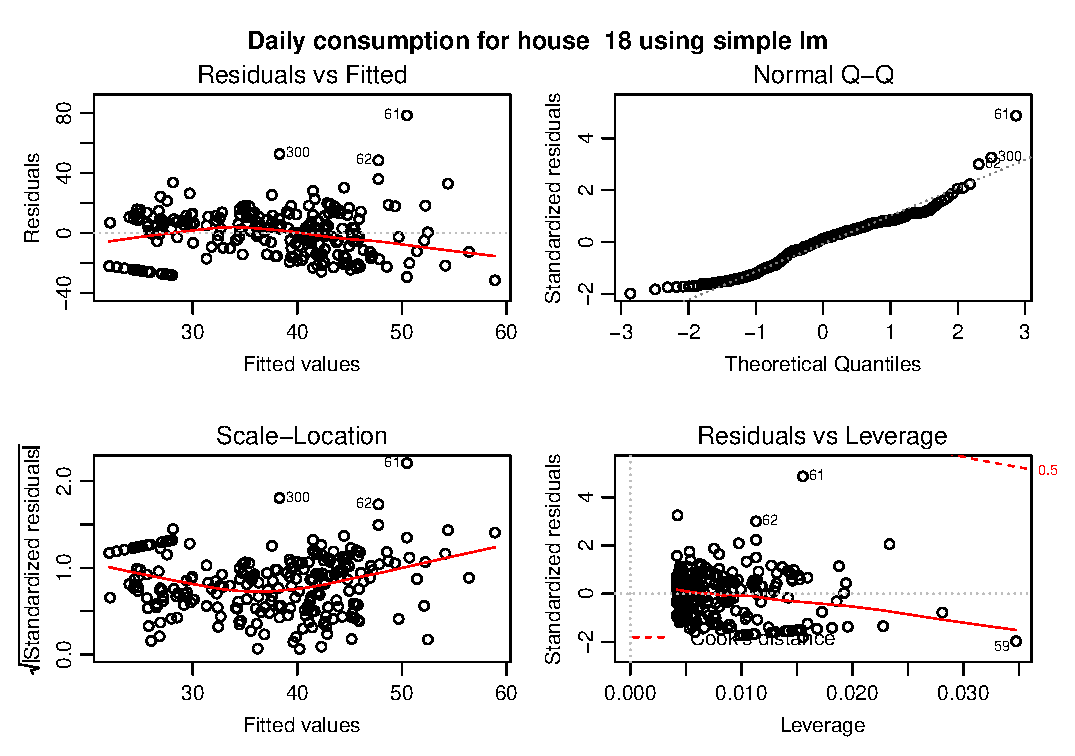
\includegraphics[width=1.\textwidth]{../../../figures/simple_lm18.eps}
    \caption{Residual plots of house 18 based on the simple linear regression model given in \cref{eq: simple}. The model assumptions of a linear regression model are not fulfilled for this specific house}
    \label{fig: simple_lm_18}
\end{figure}
\begin{figure}
    \centering
    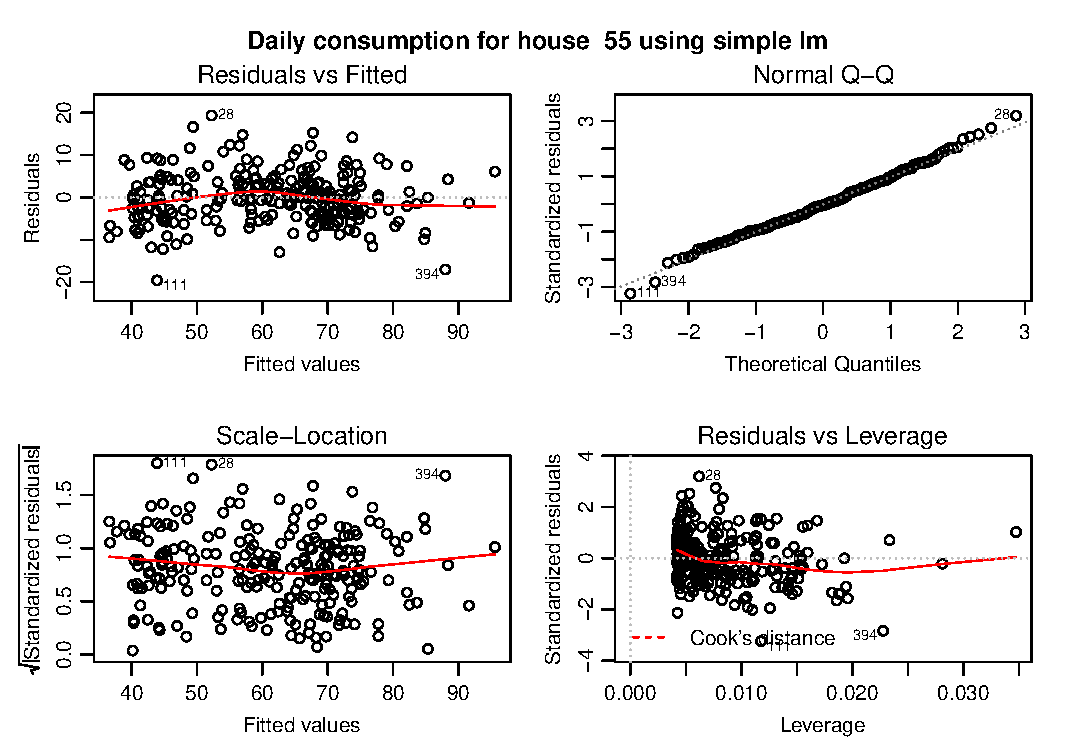
\includegraphics[width=1.\textwidth]{../../../figures/simple_lm55.eps}
    \caption{Residual plots of house 55 based on the simple linear regression model given in \cref{eq: simple}. The model assumptions of a linear regression model are overall fulfilled}
    \label{fig: simple_lm_55}
\end{figure}
In addition, a Shapiro-Wilk test and a sign test is perfomed. The hypothesis tested in the Shapiro-Wilk test is that the residuals are i.i.d and if the p-value $> 0.05$ the hypothesis can not be rejected i.e. the residuals are normally distributed. In the sign test the hypothesis is that the number of positive signs are equal to the number of negative signs, which is one of the requirements when checking for normality. If the model assumptions are also fulfilled, then the model is concluded to be valid. The p-values from both of the tests are found in \cref{tab: shapiro_simple_lm} and it is clearly seen that the majority of the simple linear regression models have residuals with p-value above the significance level at 0.05. Thus, the hypothesis is rejected and it can be concluded that the residuals are not i.i.d.
% \textcolor{blue}{Det interessante at kigge efter er de huse, hvis residuals har en mærkværdig opførsel eller den simple modellering. Som eksempel ses hus 18 i figur \ref{fig: simple_lm_18}. Det ses tydeligt, at residualerne for modellen for dette specifikke hus er gakket. Q-Q plottet ligger ikke fint langs en ret linje. Residuals vs. fitted viser en underlig opførsel, som ikke er randomly scattered.}

\subsection{Results}
The estimates from the simple linear regression models can be seen in \cref{tab: est_simple_lm}. However, since the simple models do not fulfill the model assumptions, the estimates can not be used for further analysis. \textcolor{red}{Hvad mangler der mere? haha}
%\noindent \textcolor{blue}{Overordnet kan den simple lineære regressionsmodel ikke beskrive trenden. Den antager, at temperaturen er den eneste faktor der påvirker husenes varmeforbrug. Men ved at undersøge hvorvidt model assumptions er opfyldt, så 'failer' modellen i de fleste tilfælde. Dette tyder på, at der findes flere faktorer, der påvirker varmeforbruget, hvilket selvfølgelig er forventet. Der vendes tilbage til dette i sammenligningen af de to regressionsmodeller. Når vi fitter en lineær model med en attribute, så vil man lægge linjen så summen af alle residualerne er lig 0, derfor består sign testen, men shapiro og model assumptions er ikke opfyldt, så det er ikke nok. The conclusion that the temperature is highly significant implies that this attribute will be included in the multiple linear regression model.}

\section{Multiple linear regression model}
The linear regression model is extended to a multiple linear regression model as the inclusion of several independent variables is expected to improve the model. The simple model clearly showed that the heat consumption is affected by other physical factors than temperature. Hence, a full multiple linear regression model containing the attributes given in Table \ref{tab: modeldata} is performed on the model data. The backward selection of the variables are perfomed such that the highly significant parameters from the full multiple regression model are chosen and used to develop an updated model. Since \texttt{Condition} and \texttt{PrecipitationProbability} are not normalised, they are excluded from the model. In addition, it is mentioned in Chapter 2 that the house data consists of house with observations for approximately a year and house with observations for approximately six months. Thus, the two distinct lengths of observations are modelled slighty different. There do not exist observations for winter break and spring break in the data containing the short houses. 
The wind directions are not inserted directly into the model. As mentioned in \cref{tab: weatherdata}, the wind directions are given as degrees from $0$ to $360$. But in the model the wind direction is not quantified in this way, rather it should be an effect on each of the four major directions: north, south, east and west. These will in the following be called wind direction categories. One way to classify the wind direction could be to use indicator variables, and assign each possible wind direction to a category. In this project spline functions will be used to determine the effect a certain wind direction has on the categories. As a consequence, a wind direction can have different effects on different categories. For example wind coming directly from north might have a large effect on the north category, but also a lesser effect on east and west. In real life the wind direction is often distorted close to the ground because of turbulence. Also wind directions on the border between two categories should have an effect on both. For these reasons, splines seem like a good choise for modelling the wind. \\

\subsection{Splines}
Each major direction is described by a basis spline. Together they form a spline basis, that spans the space of the wind direction. The theory on splines introduced here is based on \cite{Splines}. A spline basis is defined by a knot vector $\Xi$ and a polynomial degree $q\in \mathbb{N}$. The i'th basis spline is a function $\mathcal{N}^q_{\Xi,i}: \mathbb{R} \rightarrow \mathbb{R}$. If the spline basis should contain $n$ basic splines, then $\Xi=\{\xi_1, \xi_2,...,\xi_{n+q+1}\}$. When the knots are equidistant, the spline is uniform. Then the spline is defined by the Cox-de Boor recursion formula:

\begin{equation}
    \mathcal{N}_{\Xi,i}^0 (\xi) =
    \begin{cases}
    1 \quad \text{if} \ \ \xi_i \leq \xi \leq \xi_{i+1}\\
    0 \quad \text{otherwise}\,,
    \end{cases}
\end{equation}
for the splines of degree $0$, and for higher degrees
    \begin{equation}
        \mathcal{N}_{\Xi,i}^j(\xi) = \frac{\xi-\xi_i}{\xi_{i+j}-\xi_i}\mathcal{N}_{\Xi,i}^{j-1}(\xi) + \frac{\xi_{i+j+1}-\xi}{\xi_{i+j+1}-\xi_{i+1}} \mathcal{N}_{\Xi, i + 1}^{j-1}(\xi),
    \end{equation}
for $j=1,2,..,q$ and $i=1,2,...,n+q-j$. When the splines are uniform, the continuity of the basis splines across a knot is $q-1$. This means that the $q-1$'th derivative exists and is continuous. In this project splines of degree $2$ is used, meaning that the first derivative is continuous at every point on the spline. The splines used here are periodic. that means that after the first $n$ knots, the knot sequence starts over. For modelling the wind direction, four knots are used for the knot vector, each associated with a wind direction category.  Here they are defined as $northeast$, $southeats$, $southwest$ and $northwest$. The reason for this will be explained later in this section. For each of these knots there is a basis spline. When the degree of the splines is $2$, it means that the spline for a given knot is zero at the opposite knot. For example, when using four knots the spline peaking in the north would always be zero in the south. Higher degrees would not maintain this property. The spline basis can be seen on \cref{fig:spline_basis}. Notice that the sum of the entire spline basis at a given point always adds up to one. The figure shows how the $i$'th spline, associated with the $i$'th knot does not peak at that knot, but in the following interval. This is the reason why the knots are chosen in this way. By choosing the knots to be between the main directions north, east, south and west, this is where the basic splines peek.
\begin{figure}
    \centering
    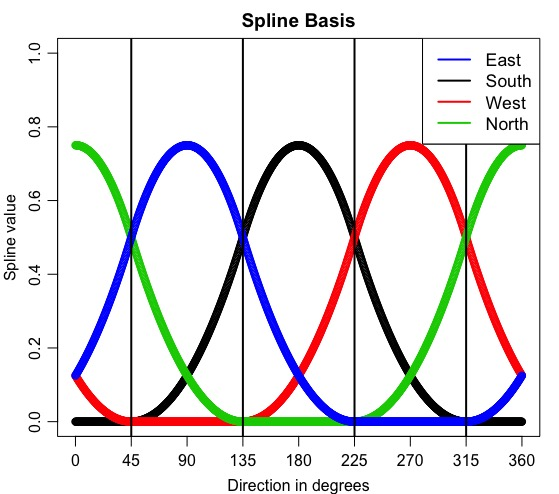
\includegraphics[width=.8\textwidth]{../../../figures/SplineBasis.jpeg}
    \caption{The spline basis used to model the wind direction. Each color is a different basis spline, and the vertical lines mark the knots}
    \label{fig:spline_basis}
\end{figure}

\noindent Now the splines can be used to represent their category in the linear regression model. At a given data point, the wind direction is given as input to each basic spline. The result is then weighted by the windspeed. The result is used as the effect of the effect of the category that spline represents. As an example, a windspeed of $2$ from the angle $135$ degrees would give the following result for the variables in the regression model: $x_N=0$, $x_E=0.5$, $x_S=0.5$ and $x_W=0$. These results can be derived from \cref{fig:spline_basis}.

\subsection{Multiple linear regression models}
The parameters included in the multiple models will be denoted as follows: Intercept (I), Temperature (T), North (N), East (E), South (S), West (W), Mean Sea Level (MSL), Solar Radiation (SR), Winter Break (WB), Spring Break (SB), Autumn Break (AB), Christmas Break (CB), Weekend (WKND), the interaction between the temperature and the different wind directions (T:N, T:E, T:S, T:W). This lead to the following two multiple linear regression models:
\begin{align}
    Y_{Q,L} = \mu & + \beta_{\text{T}}\cdot x_{\text{T}} + \beta_{\text{N}}\cdot x_{\text{N}} + \beta_{\text{E}}\cdot x_{\text{E}}+ \beta_{\text{S}}\cdot x_{\text{S}} + \beta_{\text{W}}\cdot x_{\text{W}} + \beta_{\text{MSL}}\cdot x_{\text{MSL}} \nonumber \\ & + \beta_{\text{SR}}\cdot x_{\text{SR}} + \beta_{\text{WB}}\cdot x_{\text{WB}} + \beta_{\text{SB}}\cdot x_{\text{SB}}  + \beta_{\text{AB}}\cdot x_{\text{AB}} + \beta_{\text{CB}}\cdot x_{\text{CB}} \label{eq: multi_L}  \\ & + \beta_{\text{WKND}}\cdot x_{\text{WKND}} + (\beta_{\text{T:N}} + \beta_{\text{T:E}} + \beta_{\text{T:S}} + \beta_{\text{T:W}}) \cdot x_{\text{T}} + \varepsilon \nonumber \\ \nonumber \\
    Y_{Q,S} = \mu & + \beta_{\text{T}}\cdot x_{\text{T}} + \beta_{\text{N}}\cdot x_{\text{N}} + \beta_{\text{E}}\cdot x_{\text{E}}+ \beta_{\text{S}}\cdot x_{\text{S}} + \beta_{\text{W}}\cdot x_{\text{W}} + \beta_{\text{MSL}}\cdot x_{\text{MSL}} \nonumber \\ & + \beta_{\text{SR}}\cdot x_{\text{SR}} + \beta_{\text{AB}}\cdot x_{\text{AB}} + \beta_{\text{CB}}\cdot x_{\text{CB}} + \beta_{\text{WKND}}\cdot x_{\text{WKND}} \label{eq: multi_S} \\ & + (\beta_{\text{T:N}} + \beta_{\text{T:E}} + \beta_{\text{T:S}} + \beta_{\text{T:W}}) \cdot x_{\text{T}} + \varepsilon  \nonumber
\end{align}
The models include the interaction between the temperature and the wind since it is expected that this interaction has an influence on the heat consumption. That is, it is expected that the influence of the wind is greater when the temperature is lower. In linear regression, it is desired to have as simple a model as possible, and since the models would be too complex when including all the interactions, only the interaction between the temperature and the wind is included.
\noindent The models also show that the interactions between the attribute \texttt{Holiday} and the other attributes are chosen to be excluded. The reason is that \texttt{Holiday} is used to investigate how the consumption changes during holiday periods. 

%\noindent As for the simple model, the multiple models must also be validated by investigating diagnostic plots and testing for normally distributed residuals. 
\noindent The full multiple regression models are steps of the backward selection which is why they are not validated. The purpose of this step is, as mentioned, to determine which parameters are found to be significant in the majority of the models. Hereafter, these parameters are included in a general regression model that can be used for comparing the houses performance. Before performing the models, the wind will be modified which the following section explains.

%\subsection{Validation}
%The multiple models has to fulfill several assumptions.


%\begin{figure}
%    \centering
%    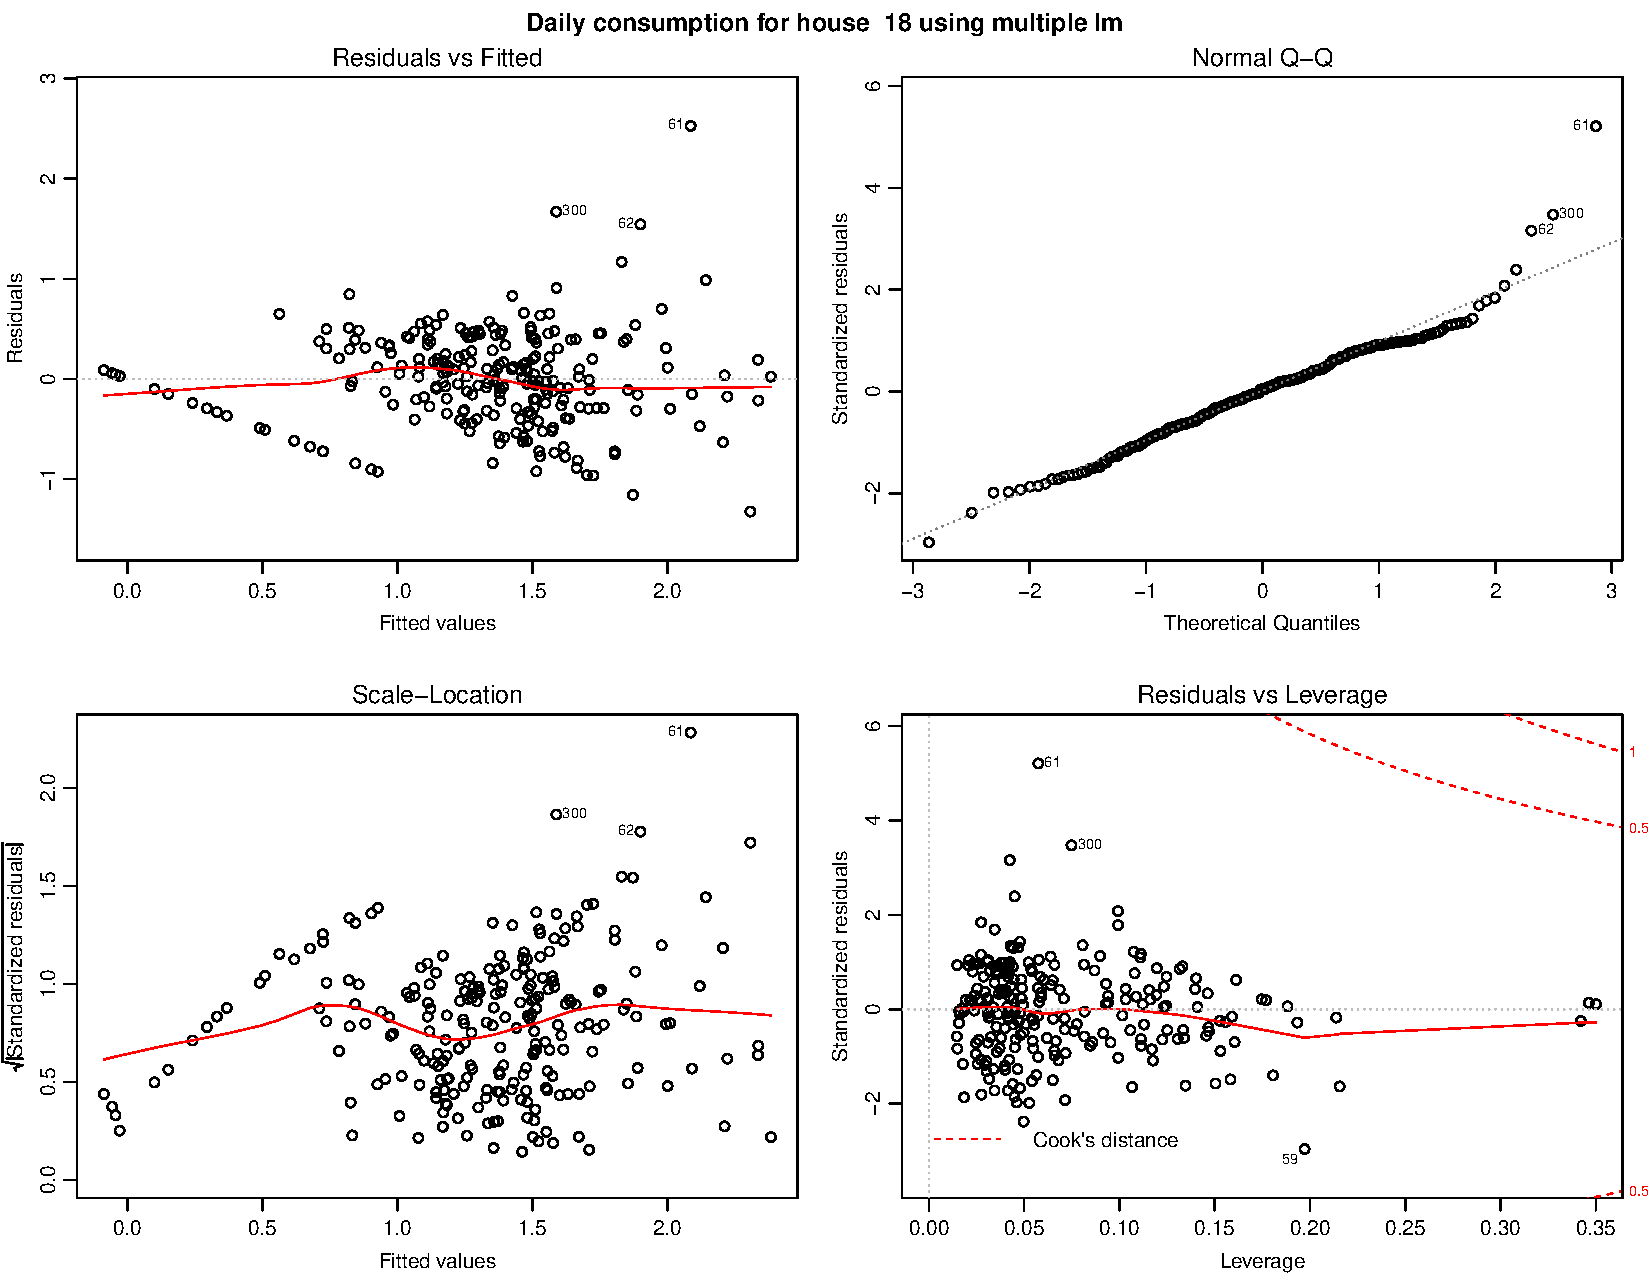
\includegraphics[width=1.\textwidth]{../../../figures/multiple_lm18L.pdf}
%    \caption{Diagnostic plot of the multiple linear regression model for long house 18}
%    \label{fig: multiple_lm18L}
%\end{figure}
%\begin{figure}
%    \centering
%    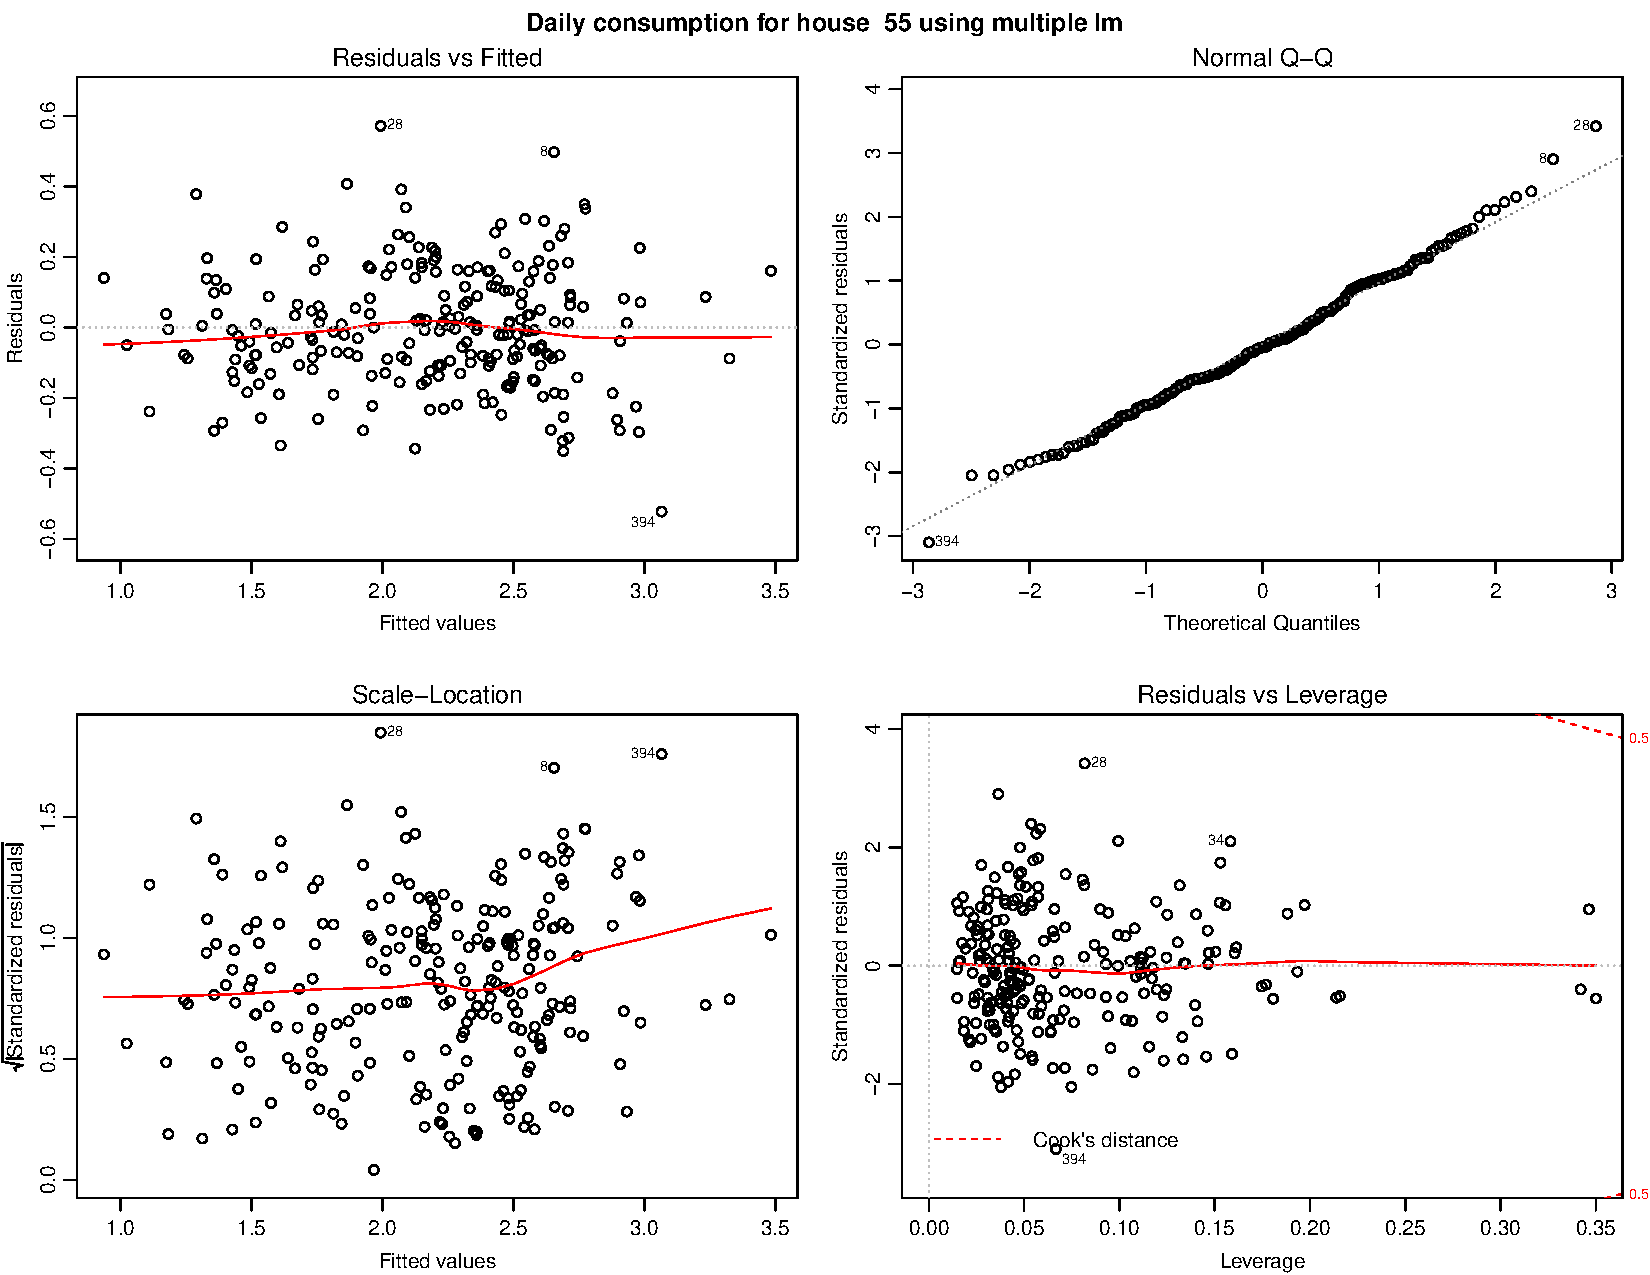
\includegraphics[width=1.\textwidth]{../../../figures/multiple_lm55L.pdf}
%    \caption{}
%    \label{fig: multiple_lm55L}
%\end{figure}


%\begin{figure}
%    \centering
%    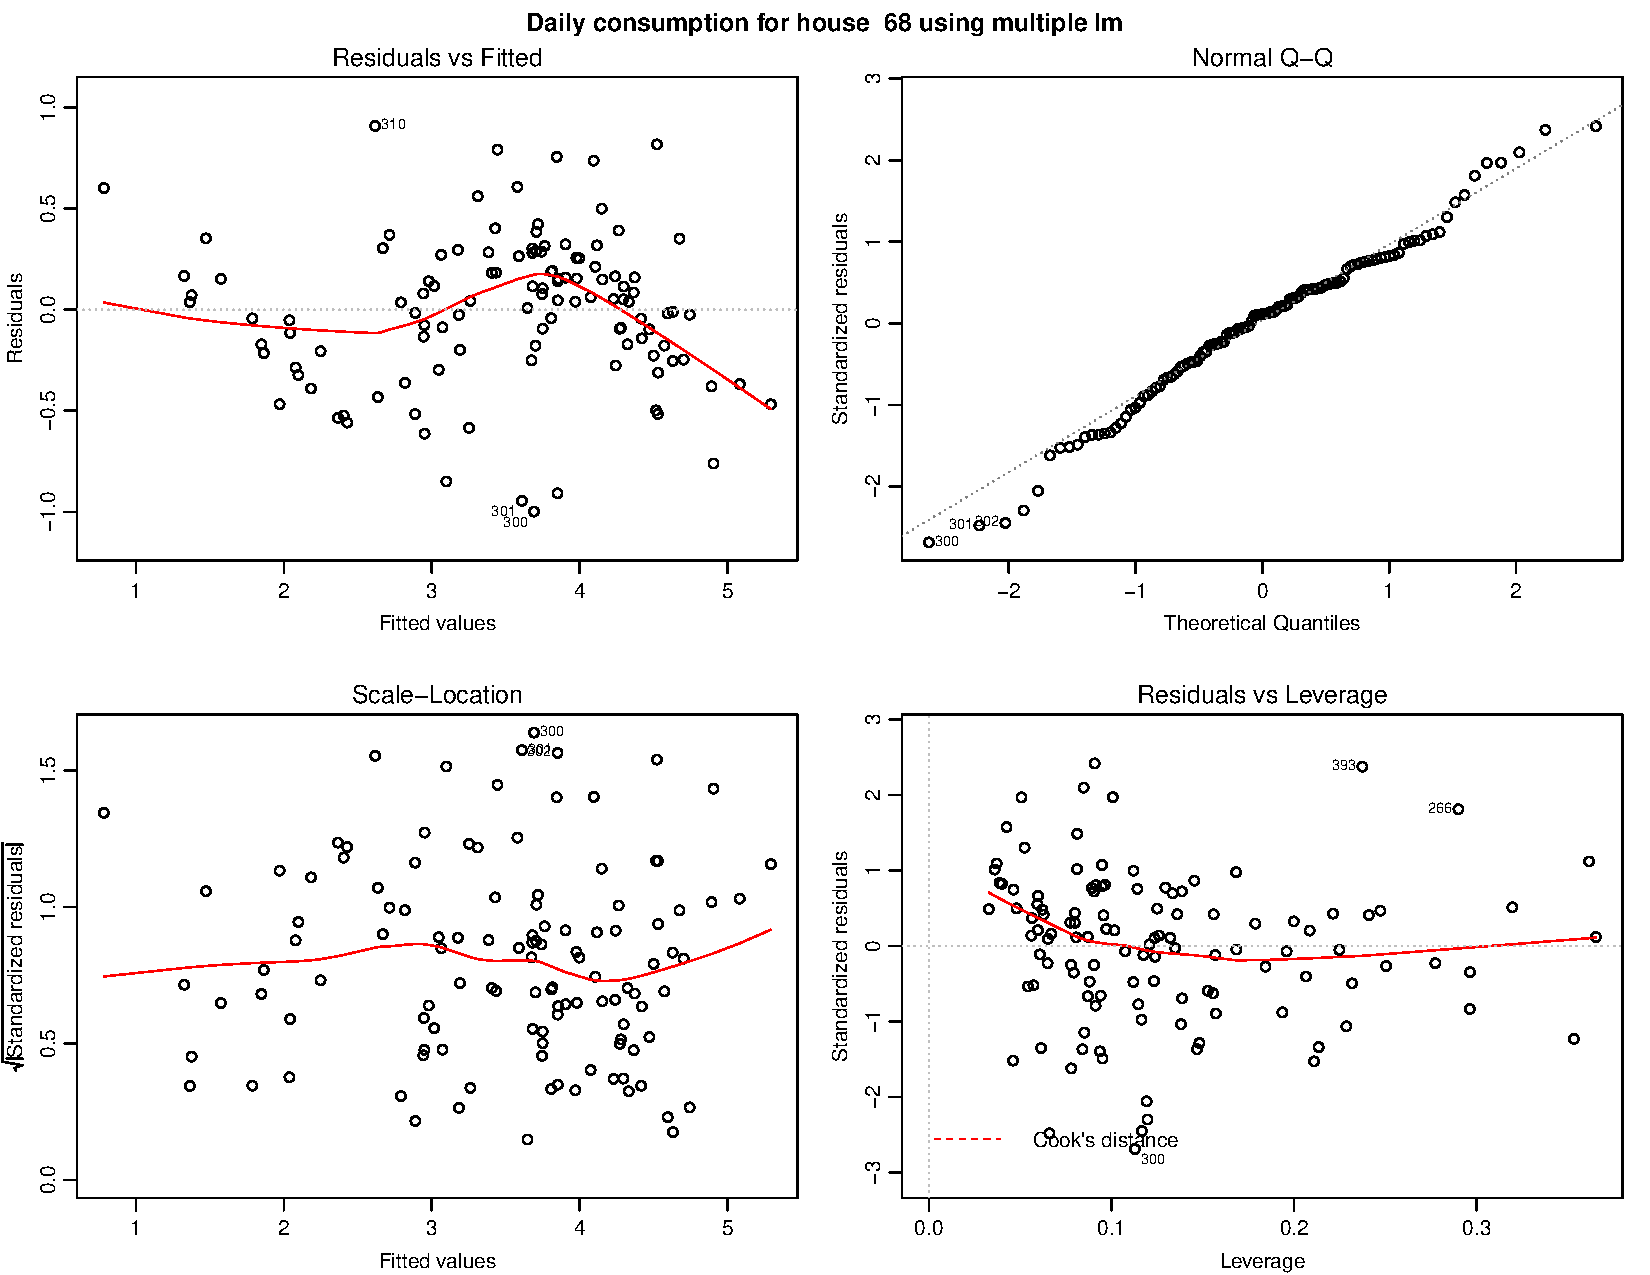
\includegraphics[width=1.\textwidth]{../../../figures/multiple_lm68S.pdf}
%    \caption{}
%    \label{fig: multiple_lm68S}
%\end{figure}


\subsection{Results}
When performing the two models given in \cref{eq: multi_L} and \cref{eq: multi_S}, without reduction, the significance of the parameters are determined and can be found in \cref{tab: lmMult_full_L}-\ref{tab: lmMult_full_S}. In addition, \cref{tab: lmMult_full_L_sum} and \cref{tab: lmMult_full_S_sum} are generated in order to determine which parameters are significant for the majority of the houses. The tables clearly show that the total of significance of the intercept, temperature, east and west as well as the interaction between temperature and west and the solar radiation occurs in more than half of the models. Thus, these are included in the general regression model. But when the influence of the wind on the consumption is examined, it does not make much sense to exclude some of these parameters. Therefore, both north, south, east and west are included as well as their interaction with the temperature. Each parameter from the different holiday attributes is not significant for enough of the models. There might have been some patterns in when the households vacationed, which the tables also indicate, but the impact on consumption is not large enough for the holidays to be included in the general model.
\begin{table}
    \centering
    \resizebox{0.70\textheight}{!}{\begin{tabular}{l|cccccccccccccccccccc}
     \hline
    & I & T & N & E & S & W & MSL & SR & WB & SB & AB & CB & WKND & T:N & T:E & T:S & T:W \\
    \hline
    Sum of *** & 5 & 41 & 0 & 18 & 2 & 24 & 6 & 22 & 3 & 3 & 1 & 5 & 4 & 0 & 1 & 7 &9 \\
    Sum of ** & 6 & 1 & 1 & 9 & 5 & 12 & 4 & 10 & 6 & 2 & 0 & 2 & 0 & 1 & 1 & 9 & 9 \\
    Sum of * & 6 & 1 & 5 & 7 & 7 & 2 & 2 & 2 & 3 & 6 & 5 & 3 & 8 & 2 & 3 & 5 & 11 \\
    \hdashline
    Total of 43 & 17 & 43 & 6 & 34 & 14 & 38 & 12 & 34 & 12 & 11 & 6 & 10 & 12 & 3 & 5 & 21 & 29 \\
    \hline
\end{tabular}}
\caption{The distribution of significant parameters from the multiple linear regression model for long houses. There are 43 long houses, thus the total of the signifance of each parameter for each house is in relation to the number of long houses}
\label{tab: lmMult_full_L_sum}
\end{table}
\begin{table}
    \centering
    \resizebox{0.7\textheight}{!}{\begin{tabular}{l|cccccccccccccccccc}
     \hline
    & I & T & N & E & S & W & MSL & SR & AB & CB & WKND & T:N & T:E & T:S & T:W \\
    \hline
    Sum of *** & 0 & 27 & 0 & 4 & 0 & 15 & 0 & 5 & 2 & 0 & 0 & 0 & 0 & 0 & 3\\
    Sum of ** & 2 & 0 & 0 & 6 & 2 & 5 & 2 & 6 & 0 & 0 & 3 & 0 & 0 & 2 & 5 \\
    Sum of * & 2 & 0 & 1 & 8 & 4 & 4 & 4 & 4 & 2 & 5 & 2 & 1 & 1 & 3 & 9 \\
    \hdashline
    Total of 27 & 4 & 27 & 1 & 18 & 6 & 24 & 6 & 15 & 4 & 5 & 5 & 1 & 1 & 6 & 17\\
    \hline
\end{tabular}}
\caption{The distribution of significant parameters from the multiple linear regression model for short houses. As for the long houses, the total of the signifance is in relation to the number of long houses}
\label{tab: lmMult_full_S_sum}
\end{table}



\section{Regression model for comparing houses}
Based on the tables illustrating the significant parameters for the long and short houses, an updated multiple linear regression model is made. The purpose of this more general model is to compare which parameters influence each house. Furthermore, houses with e.g. same area, construction year etc. can be compared. \textcolor{red}{Men gør vi overhovedet det?} The comparison model derived from \cref{tab: lmMult_full_L_sum} and \cref{tab: lmMult_full_S_sum}, becomes
\begin{align}
        Y_{Q} = \mu & + \beta_{\text{T}}\cdot x_{\text{T}} + \beta_{\text{N}}\cdot x_{\text{N}} + \beta_{\text{E}}\cdot x_{\text{E}}+ \beta_{\text{S}}\cdot x_{\text{S}} + \beta_{\text{W}}\cdot x_{\text{W}} \nonumber \\ & + \beta_{\text{SR}}\cdot x_{\text{SR}} + (\beta_{\text{T:N}} + \beta_{\text{T:E}} + \beta_{\text{T:S}} + \beta_{\text{T:W}}) \cdot x_{\text{T}} + \varepsilon. \label{eq: general_lm}
\end{align}
Likewise, the models are validated and if the assumptions are fulfilled the models can be used for comparison and predictions. The model in \cref{eq: general_lm} is expected to explain the heat consumption of the houses in a more accurate way as it takes several significant parameters into account. As mentioned, the purpose of the general model is to compare the houses for what influences their specific heat consumption and thereby the house's performance. Thus, they are not further reduced.

\subsection{Validation}
In order to determine whether the general model is valid, the diagnostic plots in \cref{fig: general_lm18L} and \cref{fig: general_lm55L} are investigated. The residuals from the model for house 18 behave quite odd and are not randomly scattered. More precisely, some of the residuals lie on a straight line, as seen in the residuals vs fitted plot. The reason for this is that the heat consumption for the house is 0 at the end of autumn, as seen in \cref{fig: daily_cons}. This results in that the estimates of the consumption for these specific points are equal to the corresponding residuals with reversed sign. It seems like this specific house can not be described by a linear regression model, which will be discussed further in Chapter \ref{chap: discussion}. On the other hand, the diagnostic plots of the residuals from house 55 are definitely improved compared to the simple model and the residuals show a randomly behavior. Overall, the diagnostic plots for the general models can be said to be fulfilled. They are not perfect but that is not expected either. There are some houses whose residuals have strange patterns, but the majority of the models can be said to be valid. Furthermore, the Shapiro-Wilk tests and the sign tests in \cref{tab: shapiro_multiple_lm} are used to determine if the residuals are normally distributed. The Shapiro-Wilk test shows that the hypothesis of normally distributed residuals for most of the models cannot be accepted. Similarly, the results of the sign tests do not indicate that the residuals can be concluded to be normally distributed. However, this can be said to be contrary to the diagnostic plots, which is quite remarkable. Therefore, this will be discussed in more detail in the comparison of the two regression models.
\begin{figure}
    \centering
    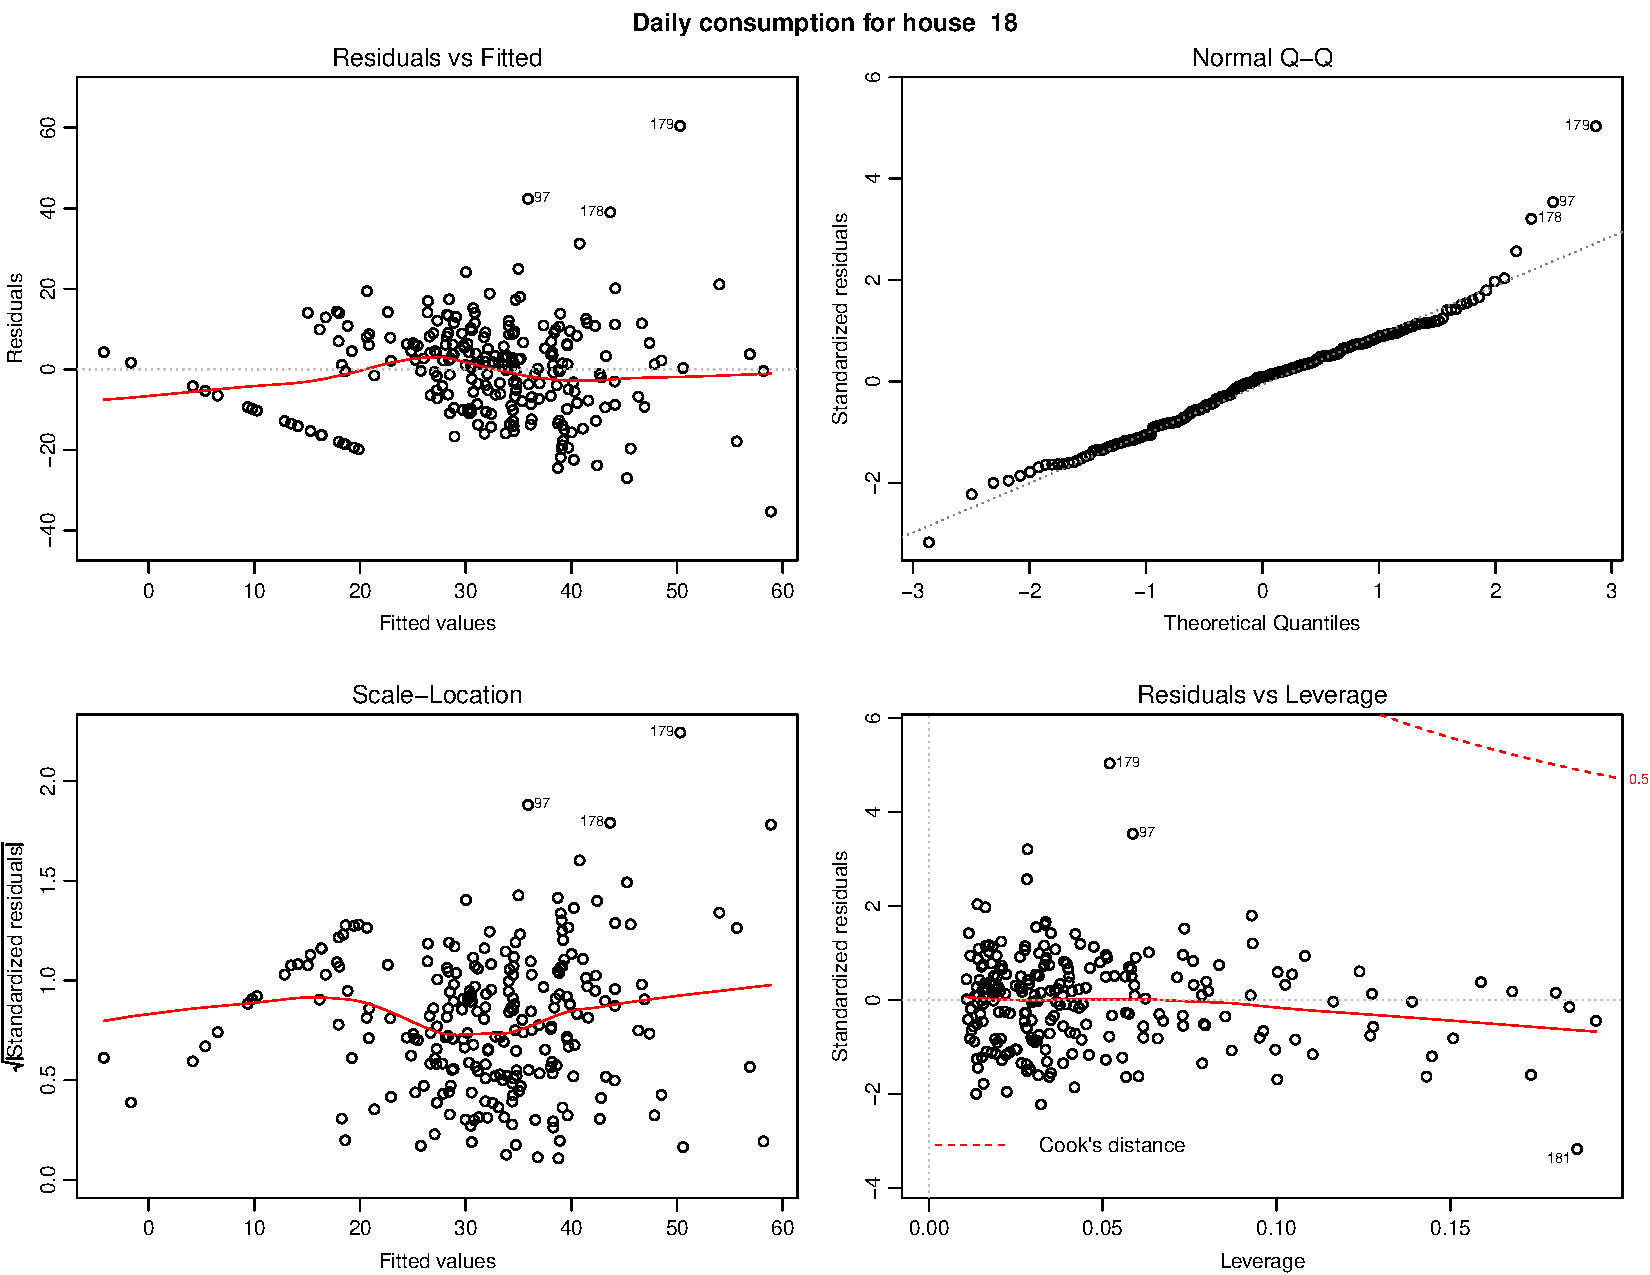
\includegraphics[width=1.\textwidth]{../../../figures/general_lm18L.pdf}
    \caption{Diagnostic plot of the general multiple linear regression model for long house 18. }
    \label{fig: general_lm18L}
\end{figure}
\begin{figure}
    \centering
    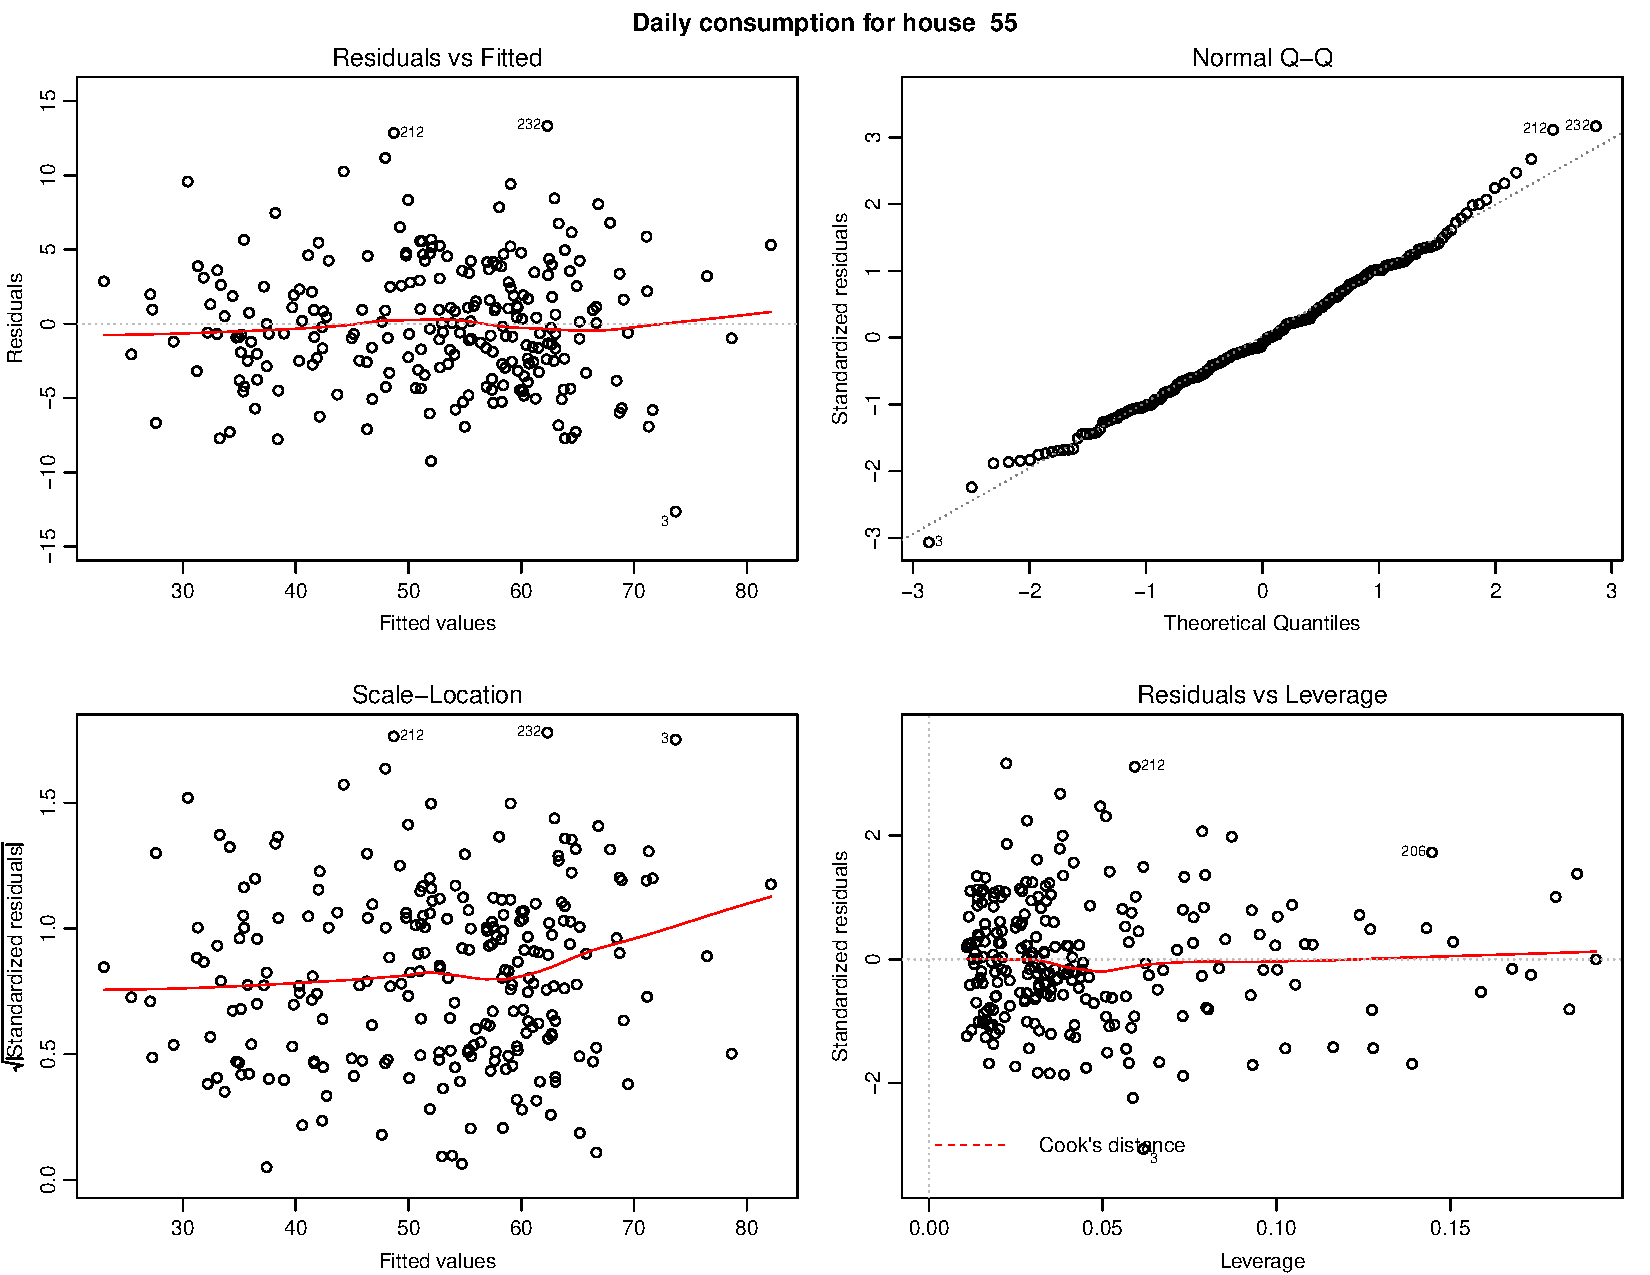
\includegraphics[width=1.\textwidth]{../../../figures/general_lm55L.pdf}
    \caption{Diagnostic plot of the general multiple linear regression model for long house 55}
    \label{fig: general_lm55L}
\end{figure}
\noindent In spite of the abovementioned, the models are concluded to somewhat fulfill the model assumptions and the estimates can be investigated further. 

\subsection{Results}
The results of the general regression model performed on each house, are illustrated in \cref{tab: lmMult_gen_L} and \cref{tab: lmMult_gen_S} with the significance of each parameter. As expected, the intercept and the temperature are highly significant in all models and with the "correct" sign. That is to say, the expected sign of the temperature is negative since the increase in the temperature will result in a decrease in the heat consumption. The attribute \texttt{SolarRadiation} effects the majority of the houses as well. The solar radiation warms the house up through the windows, so it makes sense that this has significance for how large the heat consumption is. In order to compare the houses, the temperature coefficients as well as the solar radiation coefficients are illustrated in \cref{fig: Temp_coef} and \cref{fig: Solar_coef} including a 95\% confidence interval. The influence of the temperature on house 18 is minimal but the confidence interval is quite wide compared to the houses lying close to 18. Thus, there is a large uncertainty for this specific model. Likewise, house 55 is not particularily effected by the outdoor temperature. The step response is approximately $-0.023 \ kWh/m^2$. The confidence interval is narrow, so the uncertainty for this model is quite small compared to the model for house 18. The model with the largest temperature coeffient is the one for house 63. The step response is around $-0.273 \ kWh/m^2$. This might be explained by the construction year of the house - it was build in 1920 and according to \cref{fig: bbr_hist}, it is one of the older houses. Contrary, the influence of the temperature is the lowest for house 9. The house was build in 2009, so the expectation that the house performs quite well is somewhat true \textcolor{red}{Skal det her omskrives?} When examining the coefficients in \cref{fig: Solar_coef}, the model for house 18 shows an odd behavior. The step response is positive ($0.002 \ kWh/m^2$), i.e. the heat consumption increases when the solar radiation is increased. House 55's influence from the sun is small and again the 95\% confidence interval is quite narrow. Based on this and the confidence interval showed in \cref{fig: Temp_coef}, the model for house 55 performs well and it can describe the behavior for the specific house. House 10 the most influential in terms of solar radiation. The step response is at $-0.039 \ kWh$. However, there does not exist any BBR data on this house apart from the fact that it is a commercial building so whether this behaviour is expected or not is not known.\\ 
\begin{figure}
    \centering
    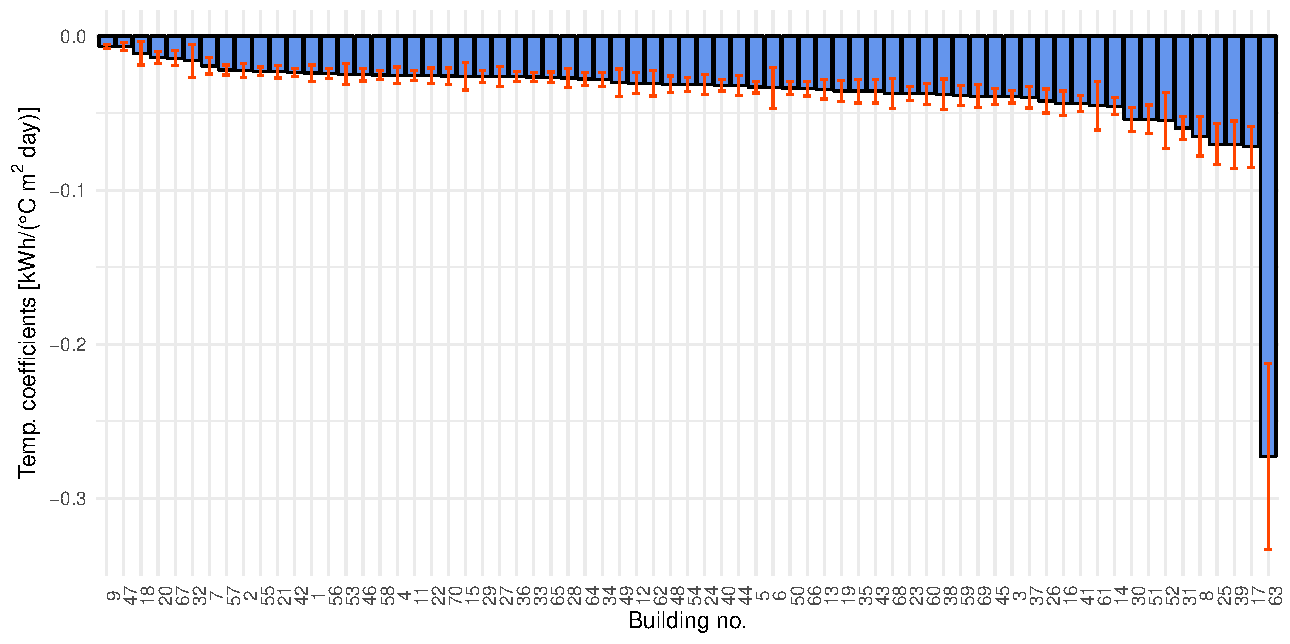
\includegraphics[width=1.\textwidth]{../../../figures/Temp_coef.pdf}
    \caption{The temperature coeffients from the general regression model. The consumption in house 63 is influenced by the temperature in a higher degree than the other houses, since the consumption decreases with 0.27 $kWh/m^2$ when the temperature increases with 1 $^{\circ}$C}
    \label{fig: Temp_coef}
\end{figure}
\begin{figure}
    \centering
    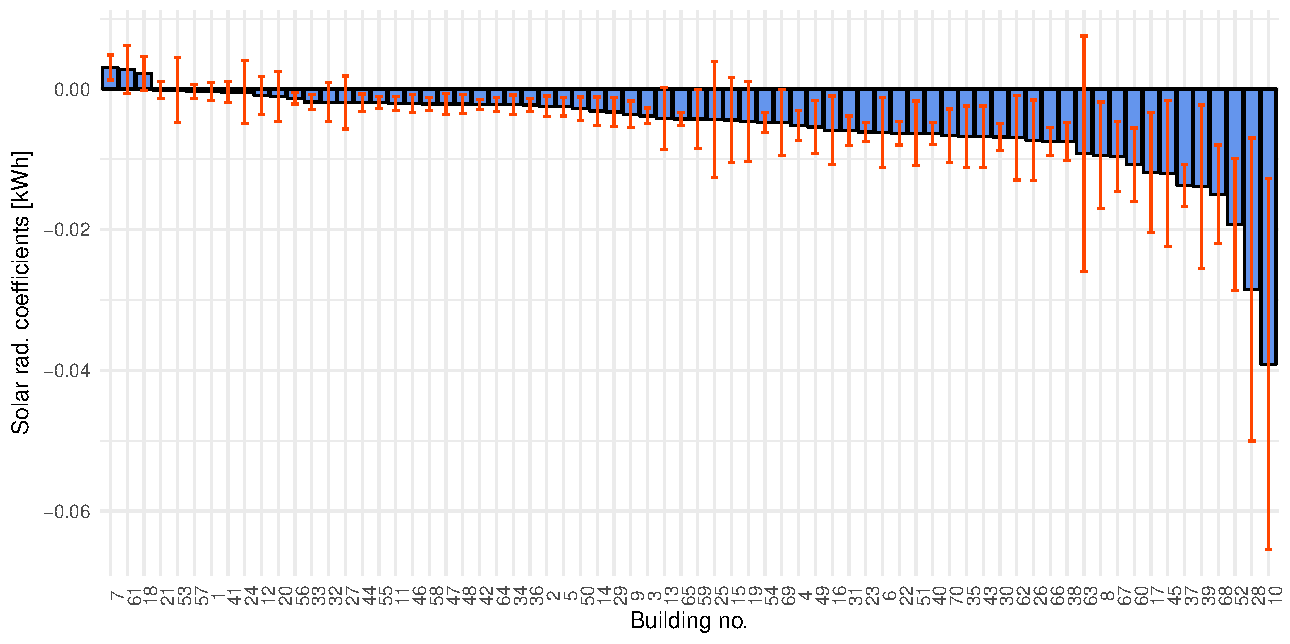
\includegraphics[width=1.\textwidth]{../../../figures/Solar_coef.pdf}
    \caption{The coeffients of the solar radiation from the general regression model. Some of the houses has a step response that increases which is not expected}
    \label{fig: Solar_coef}
\end{figure}

\noindent It can also be seen from \cref{tab: lmMult_gen_L} and \cref{tab: lmMult_gen_S} that the wind directed from East and West have great influence on the consumption of most houses. How the exact wind dependency is determined and illustrated is explained in the following about predictions.

\subsection{Predictions}
\noindent To see how well the model captures the overall behaviour of the data, it is used to make predictions for unknown data. This is done by dividing the data into a training set and a test set. Here a test set will be used containing January 2019 (31 days). The available weather data for that period is used to make predictions, which are then compared to the actual consumption. These are not one-step predictions, but 31 step predictions. This means that the model for time $t$ updates based on the prediction at time $t-1$, not the actual data. In other words, one-step predictions would be the same as predicting one step ahead 31 times and updating the available observations. The predictions are made using the function \texttt{predict} in \texttt{R} and \cref{fig: weather_pred} shows the input values used for the predictions.
\begin{figure}
    \centering
    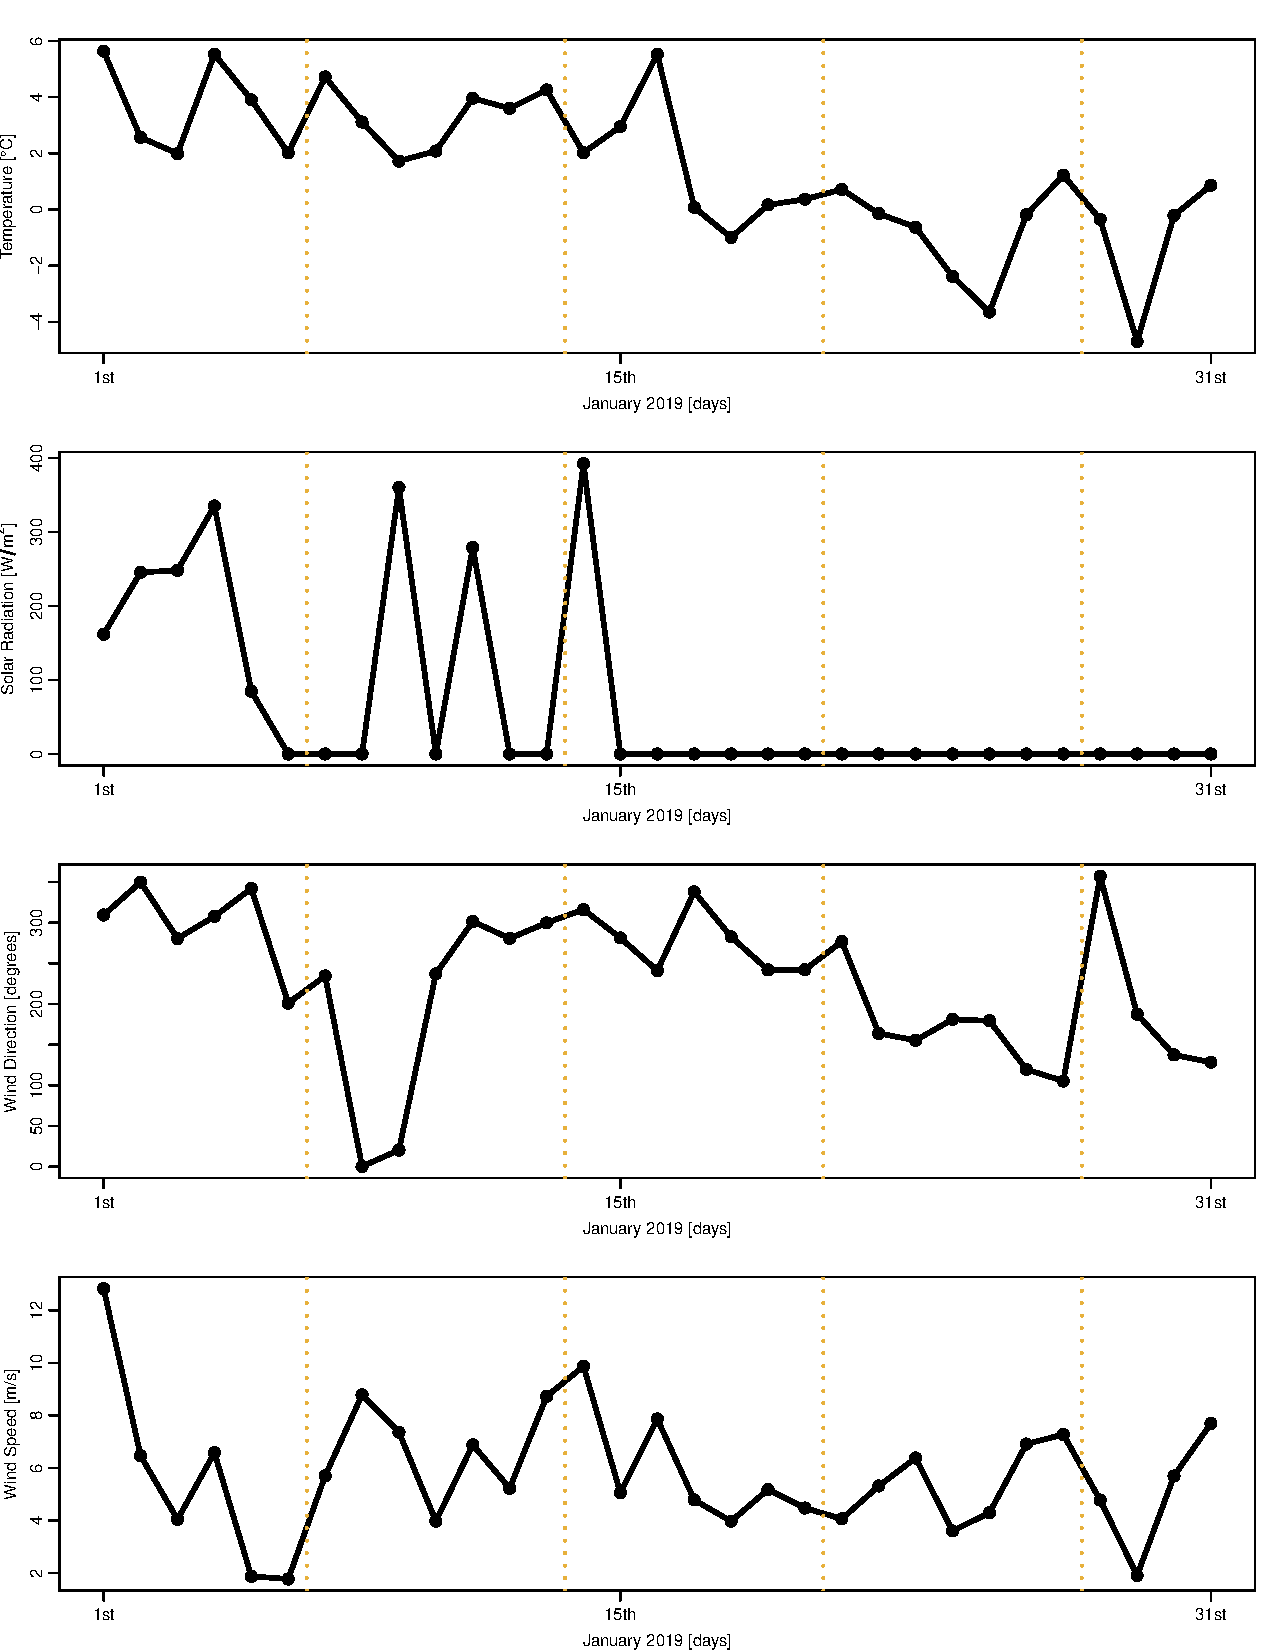
\includegraphics[width=1.\textwidth]{../../../figures/TestWeatherDays.pdf}
    \caption{The input values used for predictions of the general linear regression model. For the entire last half of January it was never sunny}
    \label{fig: weather_pred}
\end{figure}
\noindent In consistency with the other results, house 18 and 55 are used for predictions. They are illustrated in \cref{fig: lmpred_55L} and \cref{fig: lmpred_18L}.
\begin{figure}
    \centering
    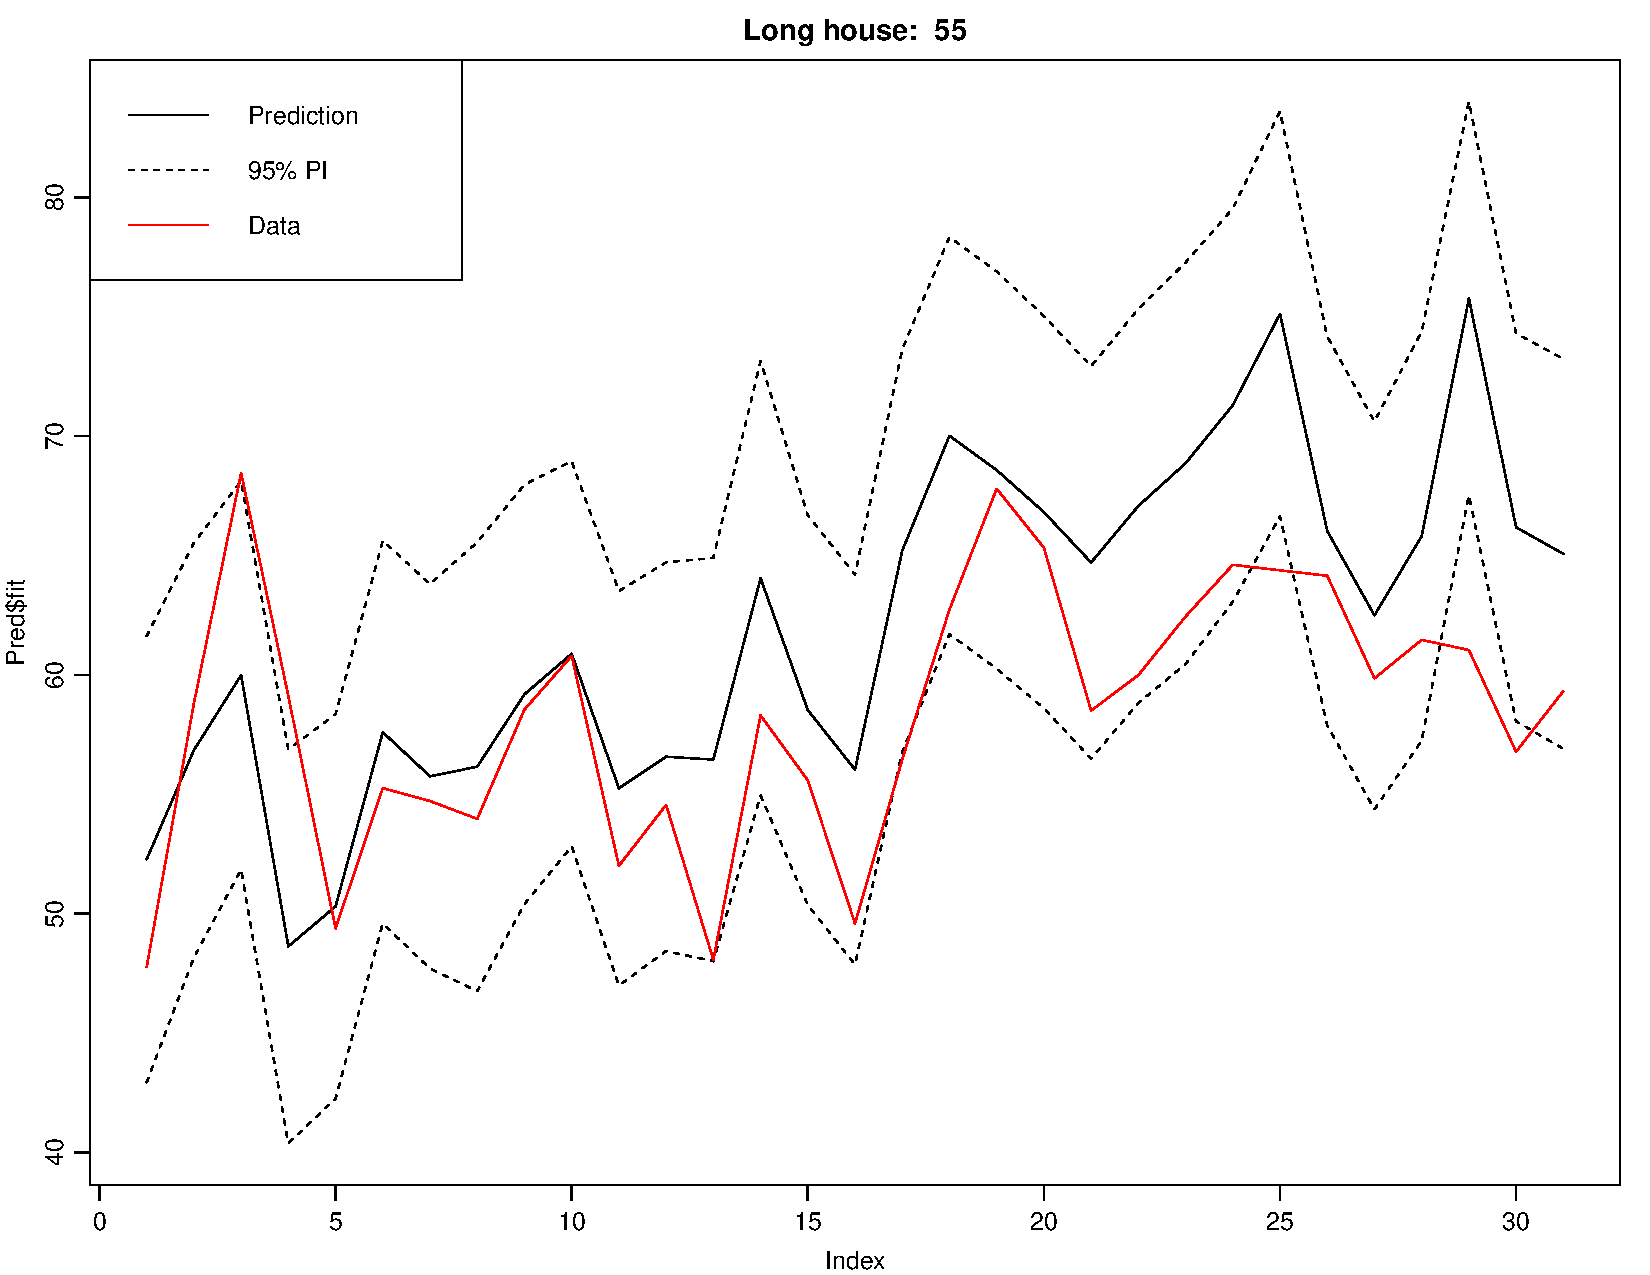
\includegraphics[width=.8\textwidth]{../../../figures/lmpred_55L.pdf}
    \caption{Predictions of the last 31 days of the model data for house 55 including a 95\% prediction interval. The model captures the behavior of this house quite well}
    \label{fig: lmpred_55L}
\end{figure}
\begin{figure}
    \centering
    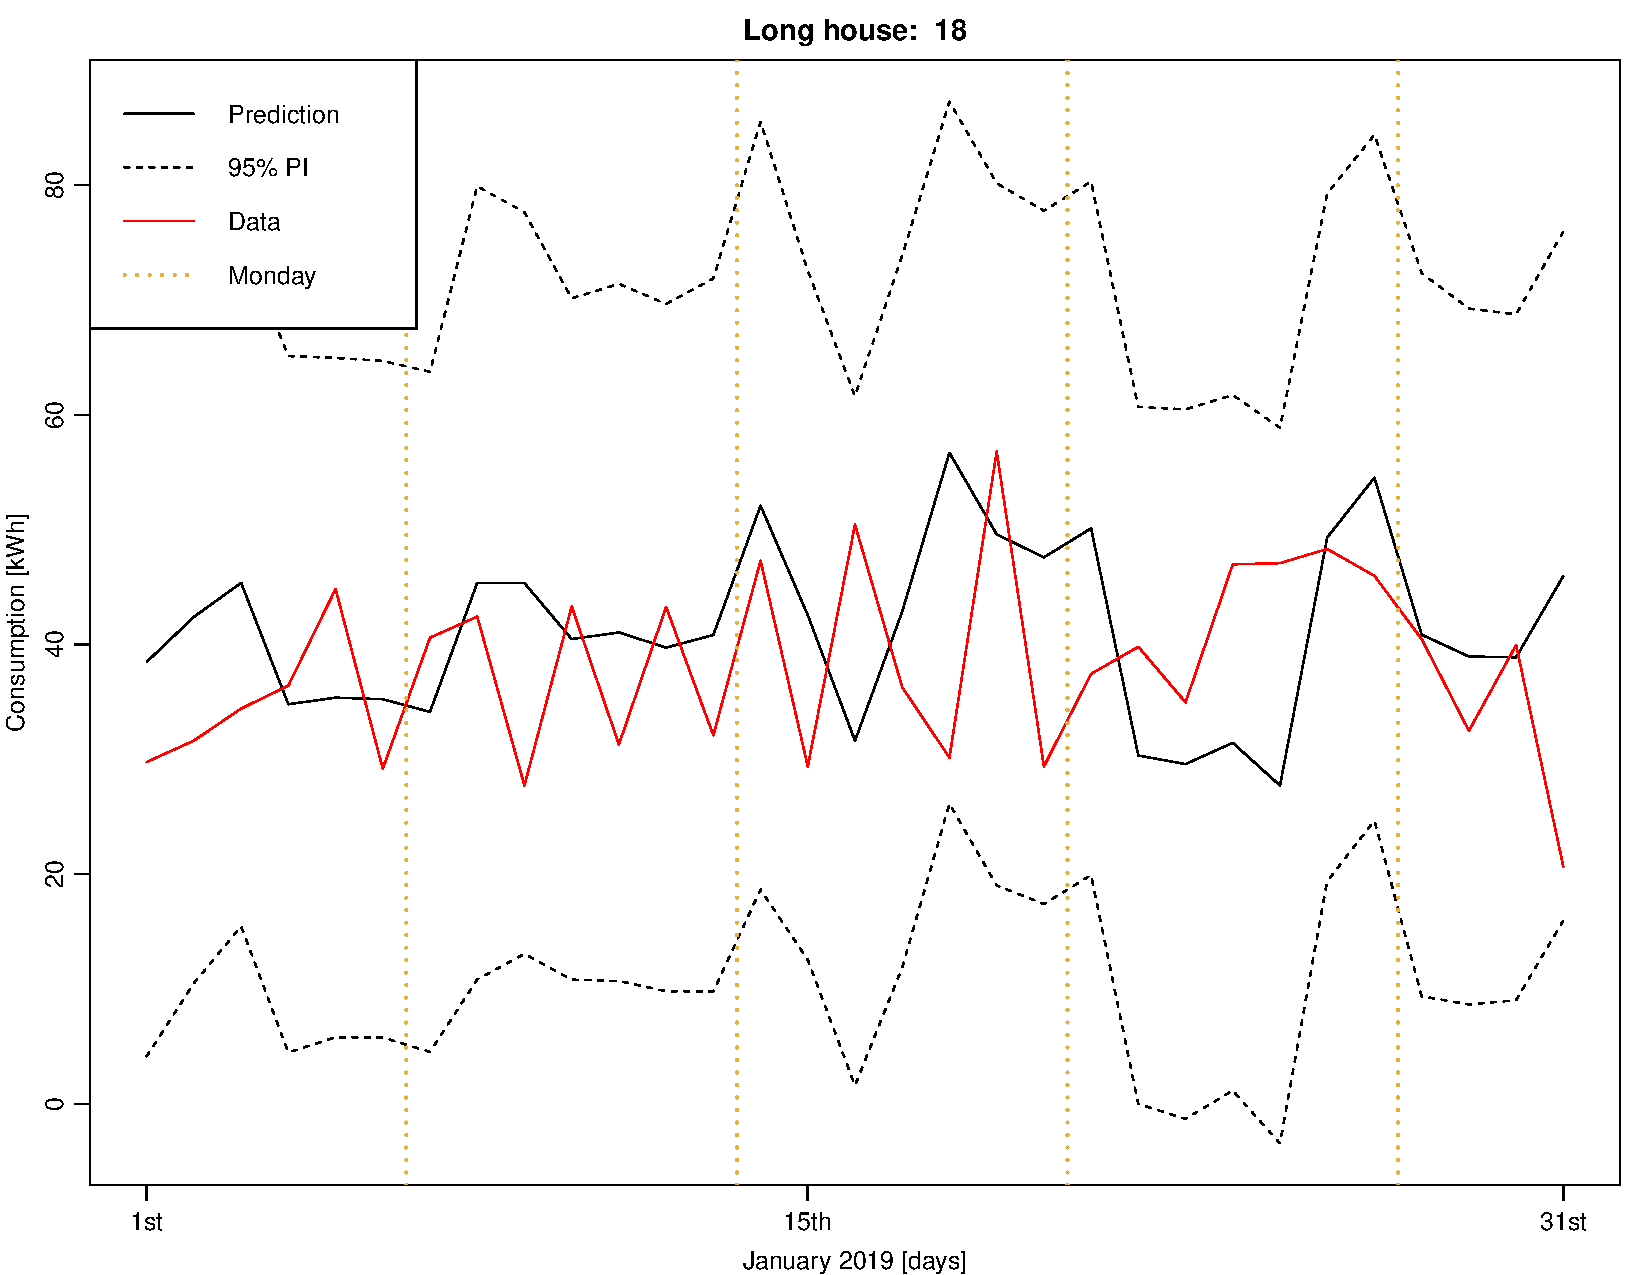
\includegraphics[width=.8\textwidth]{../../../figures/lmpred_18L.pdf}
    \caption{Predictions of the last 31 days of the model data for house 18 including a 95\% prediction interval. The model captures the behavior of this house, but the prediction interval is quite wide which indicates a large uncertainty about this model}
    \label{fig: lmpred_18L}
\end{figure}

\noindent It can be seen that the predictions for house 55 lie close to the actual data and captures the overall behaviour.  The 95\% prediction interval is narrow, which indicates that the standard deviations of this model are fairly small. Comparing the predictions to the actual consumption, the actual data is mostly inside the prediction interval. In the last couple of days the model predict spikes in the temperature that are not reflected in the observations. \cref{fig: weather_pred} indicate why the spikes occour. It seems that there are two days with particularily low temperatures coinciding with the spikes in the predictions. Low temperatures causes the model to expect higher consumption. There can be many reasons why the consumption did not spike as expected, for example the inhabitants of the house might not have been home that day to notice the temperature difference. Such things can be very hard to predict. In general, the model performs well on this house. It should be noted that there is no sun input in the input weather data for the last half of January. This makes it hard to evaluate how the sun affects the predictions.

\noindent House 18, on the other hand, does not behave quite as expected. The model has problems capturing the and the 95\% prediction interval much wider than for house 55. There is more unexplained variation in this model. The deviations in the observations cannot be explained by the input from the weather data. So even though all the observations are within the prediction interval, the model is not of much use on this house. There are other factors affecting the consumption that are not captured in the model, which is reflected in the high uncertainty.\\

\noindent The effect of the wind direction on the consumption is investigated by estimating the daily consumption for the house, for a fixed setting, where only the wind direction is changed. The setting used is a day with a temperature of $0 \degree$C, without any solar radiation, and with a wind speed of $4.27 m/s$, which is the average wind speed throughout the year. A prediction of the daily consumption is made for each wind direction and plotted with a 95\% prediction interval. \cref{fig: Wplot55} shows the wind dependency for house 55. The consumption of house 55 is by far most affected by wind from west.
\begin{figure}
    \centering
    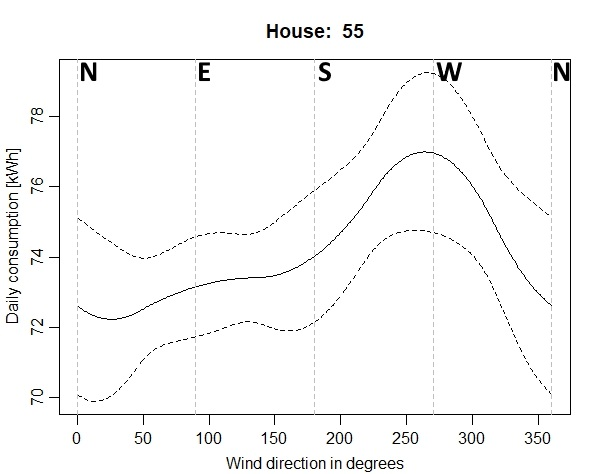
\includegraphics[width=.8\textwidth]{../../../figures/Wplot55.jpeg}
    \caption{Wind direction dependency for the consumption for house 55}
    \label{fig: Wplot55}
\end{figure}
As well as for house 55, the wind dependency is also illustrated for house 18 in \cref{fig: Wplot18}. It shows that the consumption is high when the wind comes from west and east, and low from north and south.
\begin{figure}
    \centering
    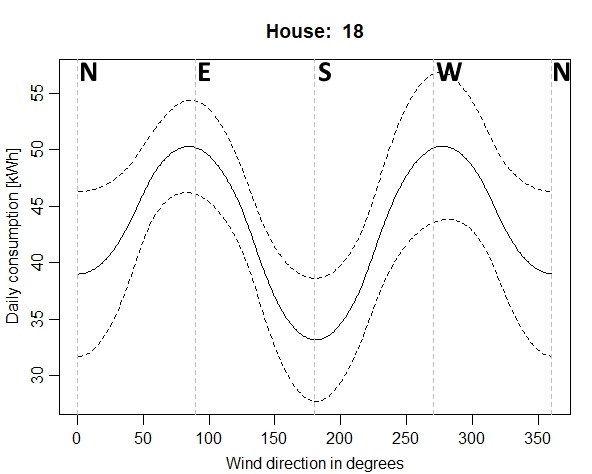
\includegraphics[width=.8\textwidth]{../../../figures/Wplot18.jpeg}
    \caption{Wind direction dependency for the consumption for house 18}
    \label{fig: Wplot18}
\end{figure}

\section{Comparison}
When looking at the results of the different tests in \cref{tab: shapiro_simple_lm}-\ref{tab: shapiro_multiple_lm}, the simple model passes the tests in more cases than the multiple model. This might be explained by the inclusion of the wind in the multiple regression model. The so-called directions are not all significant for all houses. Thus, this can affect the behavior of the residuals. On the other hand, the interpretation of the simple model shows that the temperature has a great influence on the consumption. But from a physical perspective it is known that the heat consumption is influenced by other physical phenomena as well. Hence, the simple regression model is indeed too simple. The general regression model performs as expected. It can say something about which physical phenomena affect the heat consumption of each house. The model can also predict how the expected consumption will look a month ahead. However, this is under the assumption that the weather forecasts are exact. \textcolor{red}{Ved ikke om der muligvis mangler noget her.} 

\section{Visualization of the results}
Part of this project is also to give suggestions on how the results of the analyzes can be illustrated to the users of the WATTS app. \\

\noindent The wind dependency showed in \cref{fig: Wplot55} and \cref{fig: Wplot18} can be converted to understandable plots in the following way: Each degree get one of the 3 colours, green, yellow and red, based on the 33.3\% prediction interval.  After subtracting the mean of the fit, if 0 is contained in thisinterval, the degree is coloured yellow.  If the entire interval is positive, the degree is coloured red.  Likewise if the entire interval is negative, the colour is green. Thus, the coloring is scaled according to the estimate of the wind, and that is relative to the user's own house's performance. For the users of the app, the wind direction is more intuitive as a compas on their phone.  Therefore the minimum of the lower bound of the 33.3\% prediction interval is subtracted from the fit, and then plotted as a coloured shape. The graph for the wind dependency on the consumption of house 55 and house 18 will look as follows: 
\begin{figure}
    \centering
    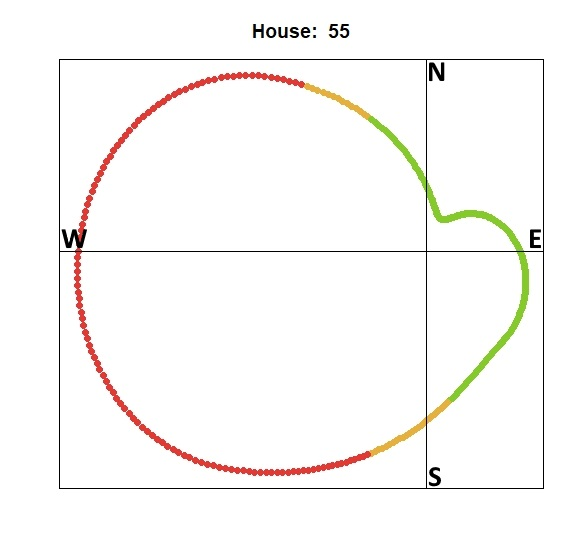
\includegraphics[width=.8\textwidth]{../../../figures/WKplot55.jpeg}
    \caption{Relative wind direction dependency for the consumption for house 55}
    \label{fig: WKplot55}
\end{figure}
\begin{figure}
    \centering
    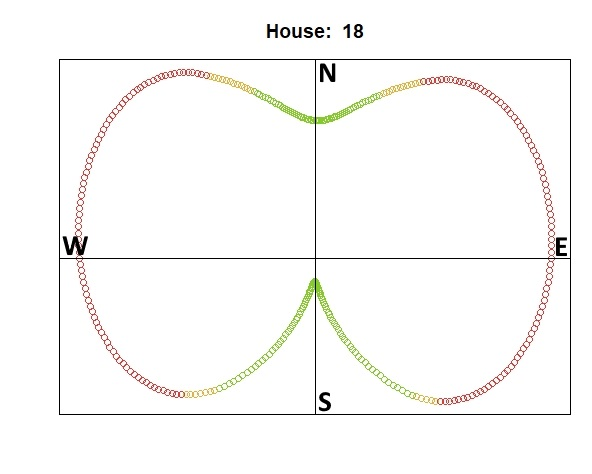
\includegraphics[width=.8\textwidth]{../../../figures/WKplot18.jpeg}
    \caption{Relative wind direction dependency for the consumption for house 18}
    \label{fig: WKplot18}
\end{figure}
The red colour indicates where the house is most influential where the consumer must be most attentive in relation to e.g. replacement of windows or better insulation. \cref{fig: WKplot55} shows that the heat consumption in house 55 increases when the wind is coming from the west. Likewise, \cref{fig: WKplot18} shows that the heat consumption increases when the wind is blowing from west and also east. These illustrations are relative to the performance of each house. It is difficult to weigh the wind directions precisely when the data does not contain information about the location of the houses which is discussed in Chapter \ref{chap: discussion}. 
%The coloring is scaled according to the estimate of the wind, and that is relative to the user's own house's performance. \textcolor{red}{ref} shows that the heat consumption for house 55 is most affected when the wind comes from west. \textcolor{red}{Kan godt være boys lige skal kommentere lidt på det her.}
\noindent \cref{fig: lmpred_55L} and \cref{fig: lmpred_18L} are also colorized with red, yellow and green. This coloring is distributed so that there is an equal probability that the heat consumption lies in one of the three areas, ie. the areas are weighted $\frac{1}{3}$ each. The red area indicates that the heat consumption exceeds the expected consumption which will result in the consumer having to pay more. If, on the other hand, the consumption is in the green area, the customer consumes less than expected and thus has to pay less than the budget. As can be seen in \cref{fig: lmpred_col_55L} for house 55, it is only in early January that the consumption exceeds the expected. Otherwise, the consumption is around the expected and for most days it is below. To be able to clarify the daily consumption even more,every day in January 2019 can be represented as a pillar, resulting in \cref{fig: lmpred_hist_55L}. As mentioned, the consumption for house 55 is most often below the expected consumption, as the bar graph clearly shows with the majority of the pillars colored green. These two suggestions for the WATTS app have also been tried on house 18. The previously mentioned oscillating behavior is clearly seen in \cref{fig: lmpred_col_18L}. This shows the consumer that they should probably have an expert investigating the house further. The bar graph in \cref{fig: lmpred_hist_18L} shows that the pillars changes colors almost every day. Once again,it can be seen that the heat consumption in house 18 has a very strange behavior.
\begin{figure}
    \centering
    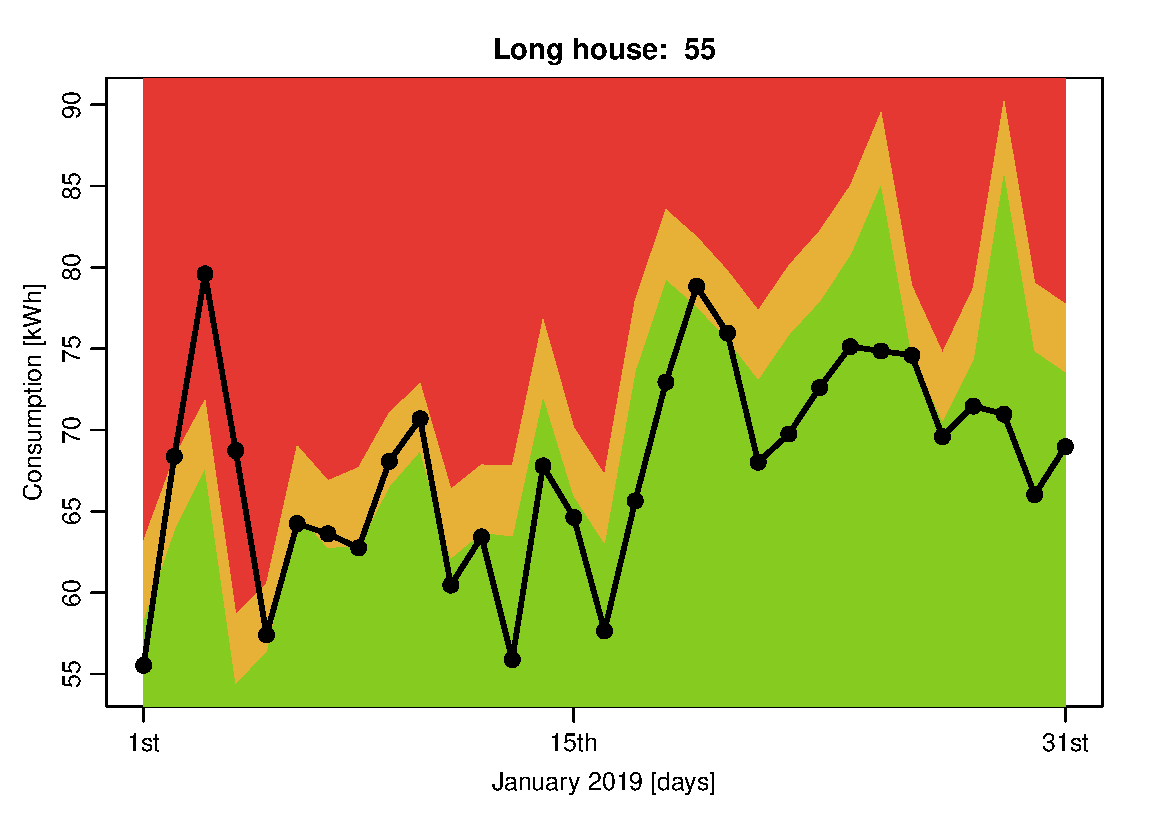
\includegraphics[width=.8\textwidth]{../../../figures/lmpred_col_55L.eps}
    \caption{This is another way of visualizing \cref{fig: lmpred_55L}. The data is the black line, and the colours show how the house performs compared to the predictions}
    \label{fig: lmpred_col_55L}
\end{figure}
\begin{figure}
    \centering
    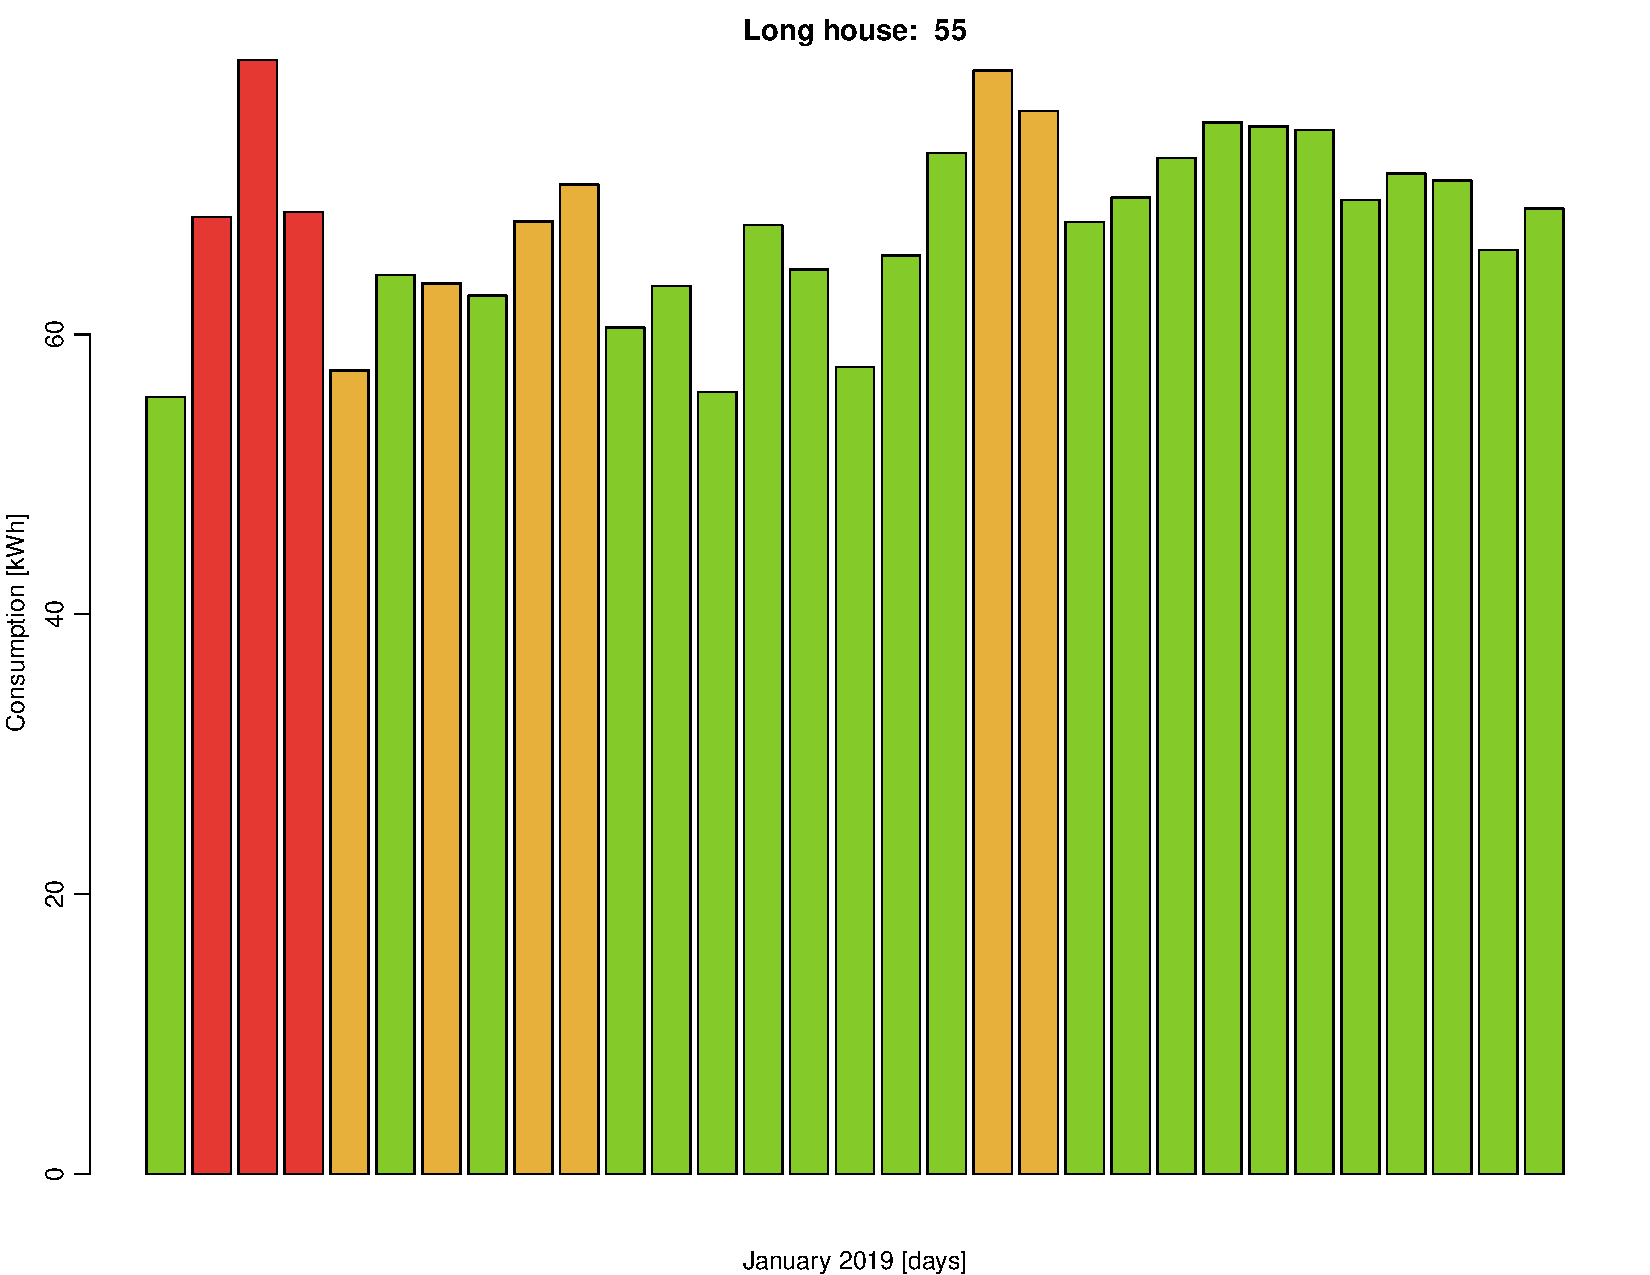
\includegraphics[width=.8\textwidth]{../../../figures/lmpred_hist_55L.pdf}
    \caption{This plot visualizes the consumption of house 55. Each bar is coloured based on where the observation is on \cref{fig: lmpred_col_55L}}
    \label{fig: lmpred_hist_55L}
\end{figure}

\begin{figure}
    \centering
    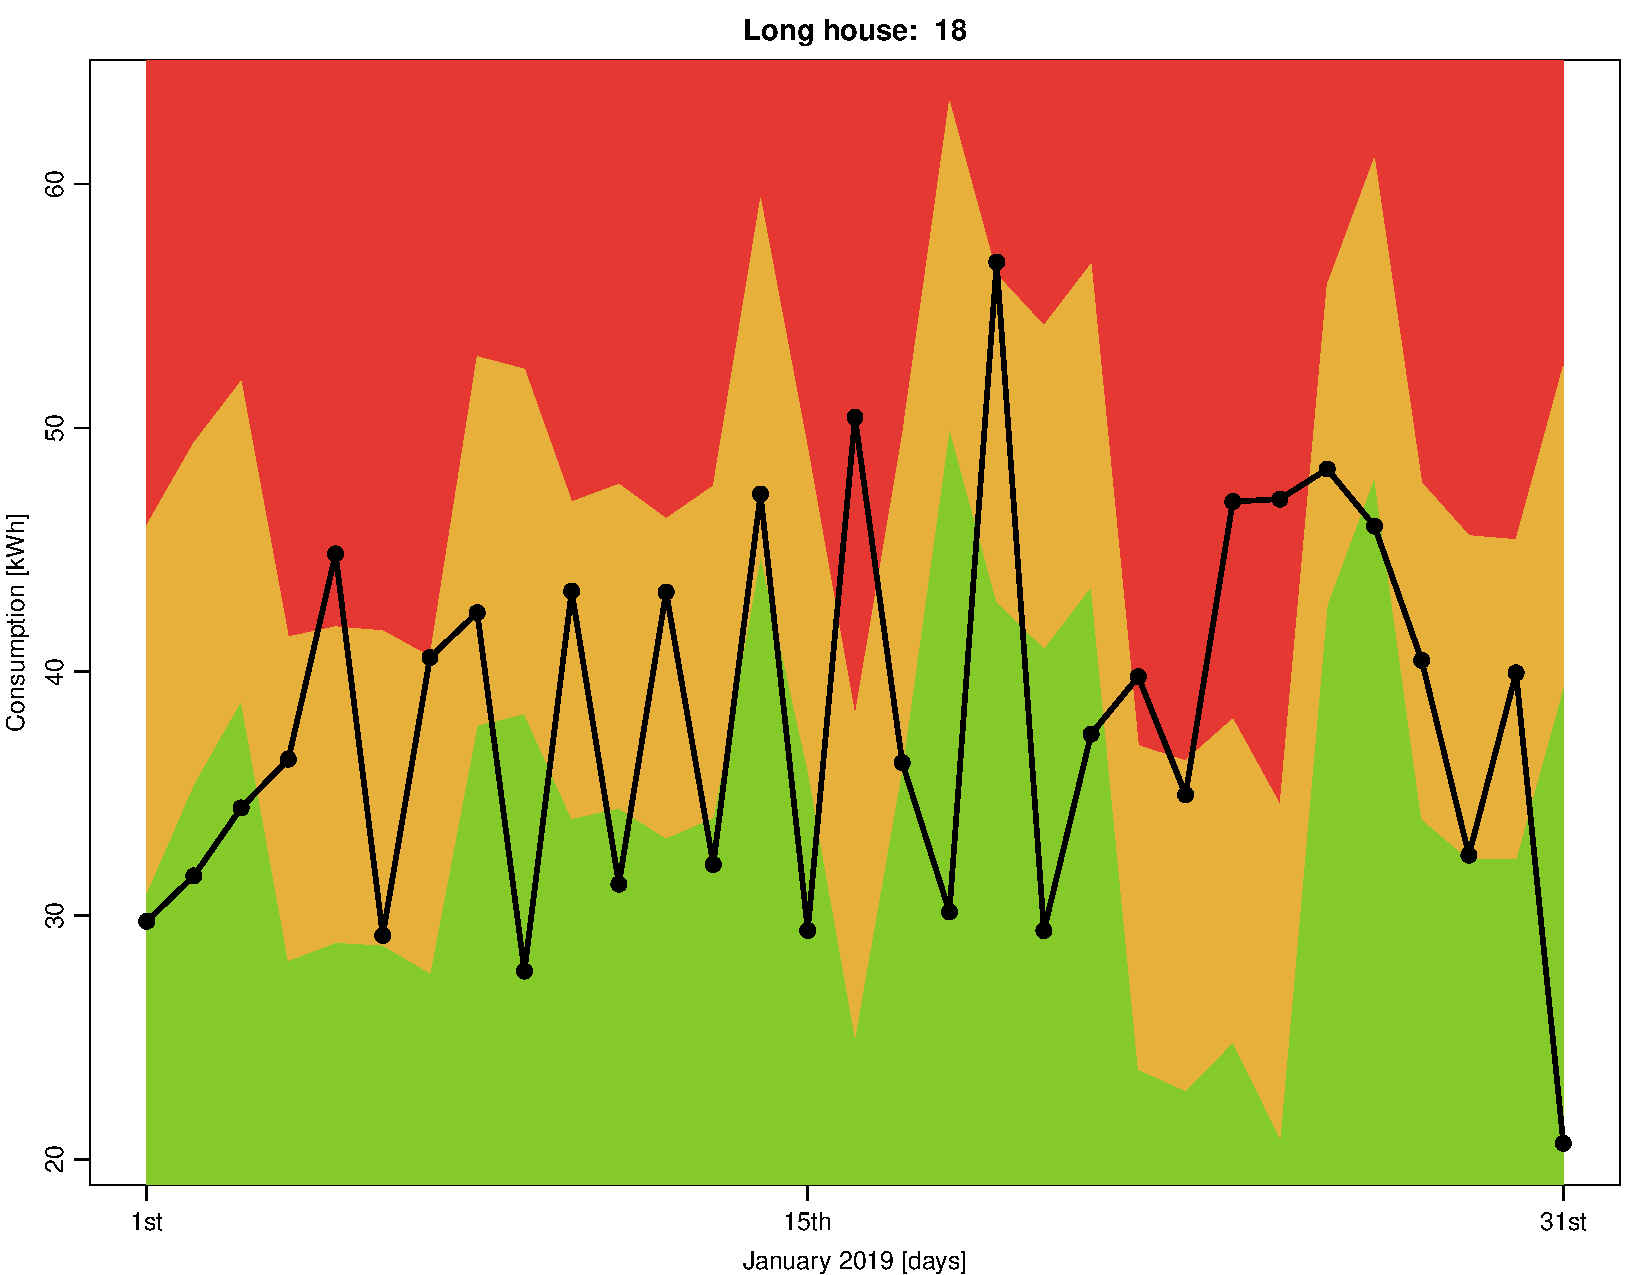
\includegraphics[width=.8\textwidth]{../../../figures/lmpred_col_18L.pdf}
    \caption{This is another way of visualizing \cref{fig: lmpred_18L}. The data is the black line, and the colours show how the house performs compared to the predictions}
    \label{fig: lmpred_col_18L}
\end{figure}
\begin{figure}
    \centering
    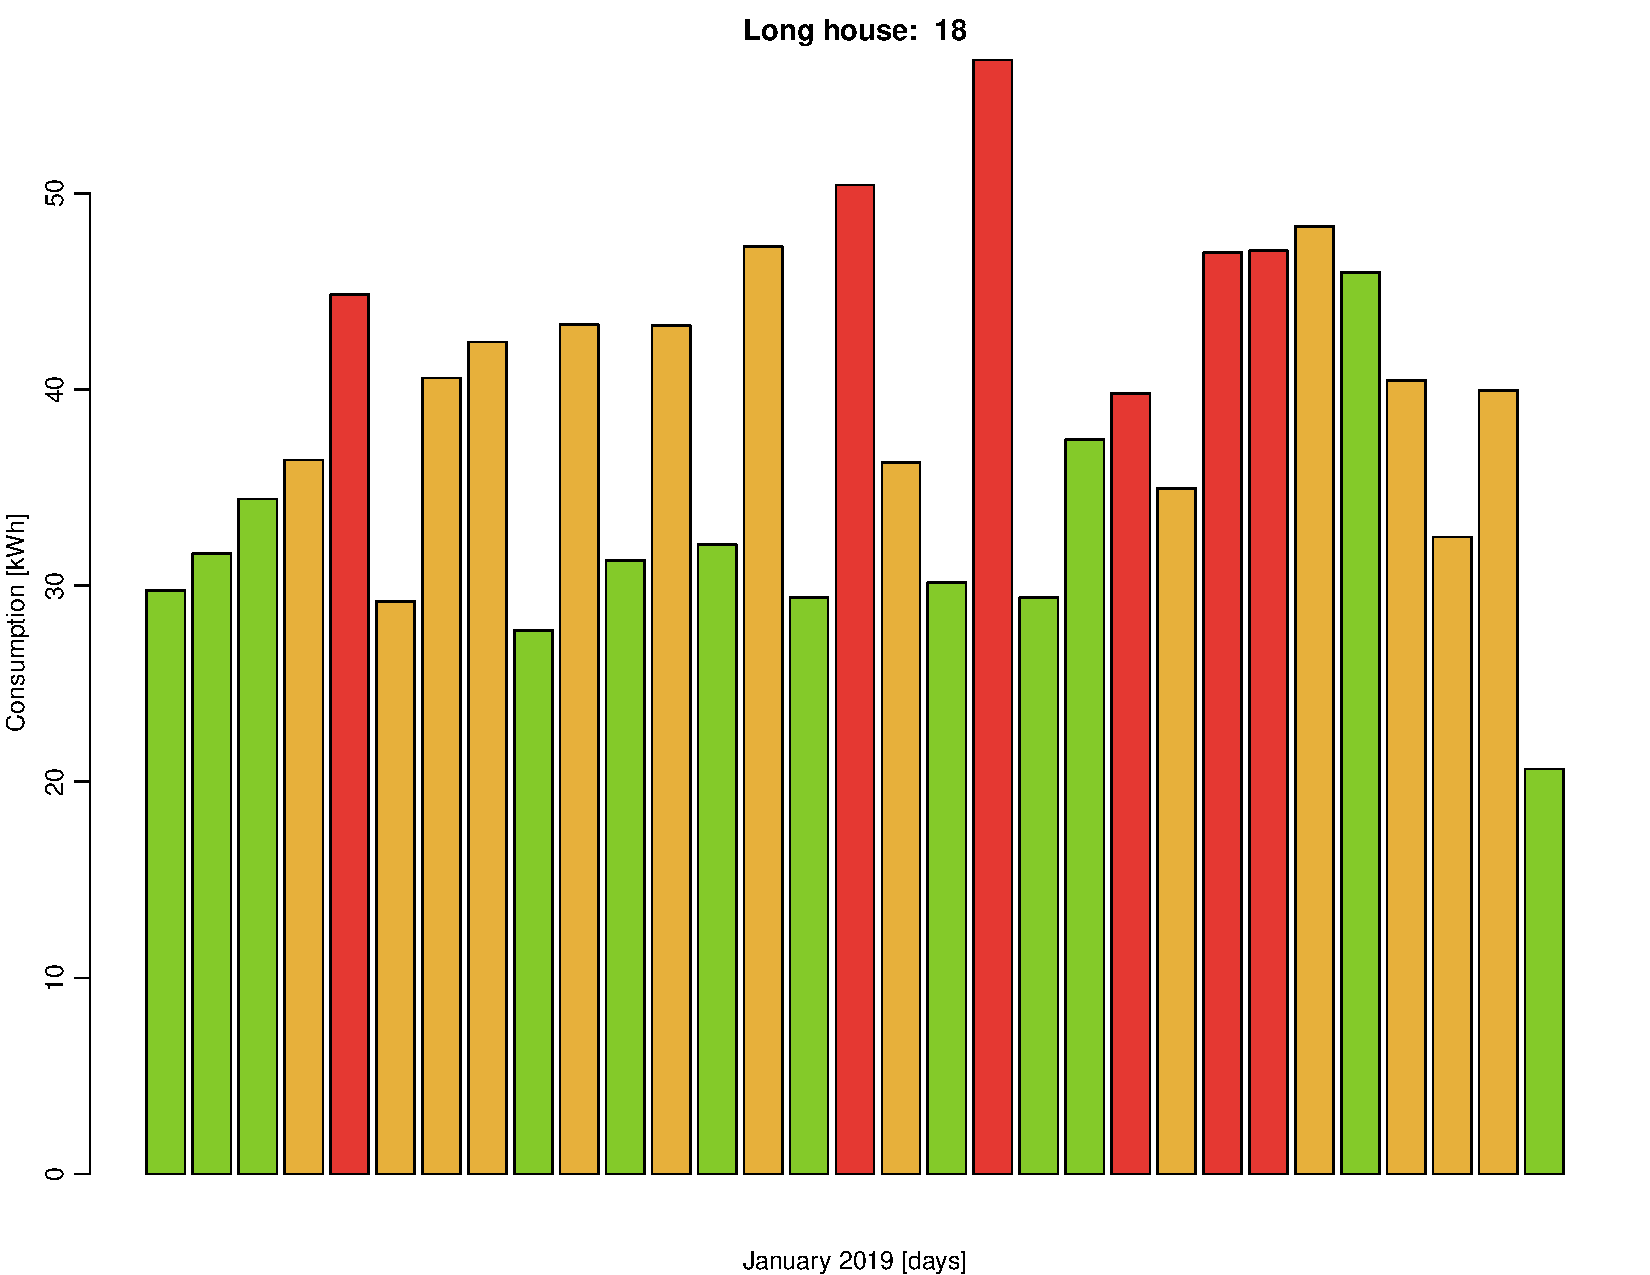
\includegraphics[width=.8\textwidth]{../../../figures/lmpred_hist_18L.pdf}
    \caption{This plot visualizes the consumption of house 18. Each bar is coloured based on where the observation is on \cref{fig: lmpred_col_18L}}
    \label{fig: lmpred_hist_18L}
\end{figure}
